\documentclass[serif, aspectratio=169, 10pt]{beamer}

% Essential packages
\usepackage{booktabs}
\usepackage{hyperref}
\usepackage{graphicx}
\graphicspath{{figures/}}

% Metropolis theme
\usetheme{metropolis}

% Colors
\definecolor{dimwhite}{rgb}{0.99, 0.99, 0.99}
\definecolor{charcoal}{rgb}{0.21, 0.27, 0.31}
\definecolor{slategray}{rgb}{0.44, 0.5, 0.56}
\definecolor{dimgray}{rgb}{0.41, 0.41, 0.41}

% Beamer colors
\setbeamercolor{background canvas}{bg=white}
\setbeamercolor{frametitle}{bg=dimwhite, fg=charcoal}
\setbeamercolor{progress bar}{fg=slategray, bg=fg!50!black!30}

% Item shapes
\setbeamertemplate{itemize items}[triangle]
\setbeamertemplate{itemize subitem}[circle]

% Margins
\setbeamersize{text margin left=7mm, text margin right=7mm}

% Title info
\title{Optimal Subsidy Design in Natural Disaster Insurance Markets: Evidence from NFIP}
\author{Anna Li and Vendela Norman}
\institute{NYU Stern}

% Revised 2026-09-21. Every number on the data slides comes from analysis.dta (SFHA homes,
% FL LA TX, 2009-2025) unless a comment on the frame says otherwise. Figures are the PNGs in
% output/figures, produced by the scripts named in the comment above each frame. Comments
% starting with "Q:" answer the bracketed questions in the 09-08 draft.

\begin{document}

\begin{frame}
\titlepage
\end{frame}

% =============================================================================
\section{Motivation and setting}
% =============================================================================

\begin{frame}{Motivation}
\begin{itemize}
    \item Natural disasters cause large economic damages, and losses will grow as the climate changes
    \begin{itemize}
        \item Flooding is the costliest: \$32 billion in expected annual losses, projected to rise 26\% by 2050 (Wing et al.\ 2022)
        \item Counting indirect costs, flooding costs the U.S. \$180--500 billion a year (Joint Economic Committee 2024)
    \end{itemize}
    \item Adapting to rising risk requires costly investments in the housing stock
    \item These investments are likely under-provided, in part because subsidized insurance mutes their return
    \item Incentivizing adaptation is a second-best problem: efficiency against affordability
\end{itemize}
\end{frame}

% Figure: descriptives/scratch/nfip_claims_timeseries.do -> output/figures/nfip_claims_by_year.png
% (all NFIP claims nationwide by year of loss, 2023 dollars, OpenFEMA claims file).
% Candidates still to source for this section: annual U.S. flood losses (NOAA billion-dollar
% events, flood + tropical cyclone) and the Wing et al. (2022) 2020-2050 projection.
\begin{frame}{Motivation: Flood Losses Are Large and Lumpy}
\centering
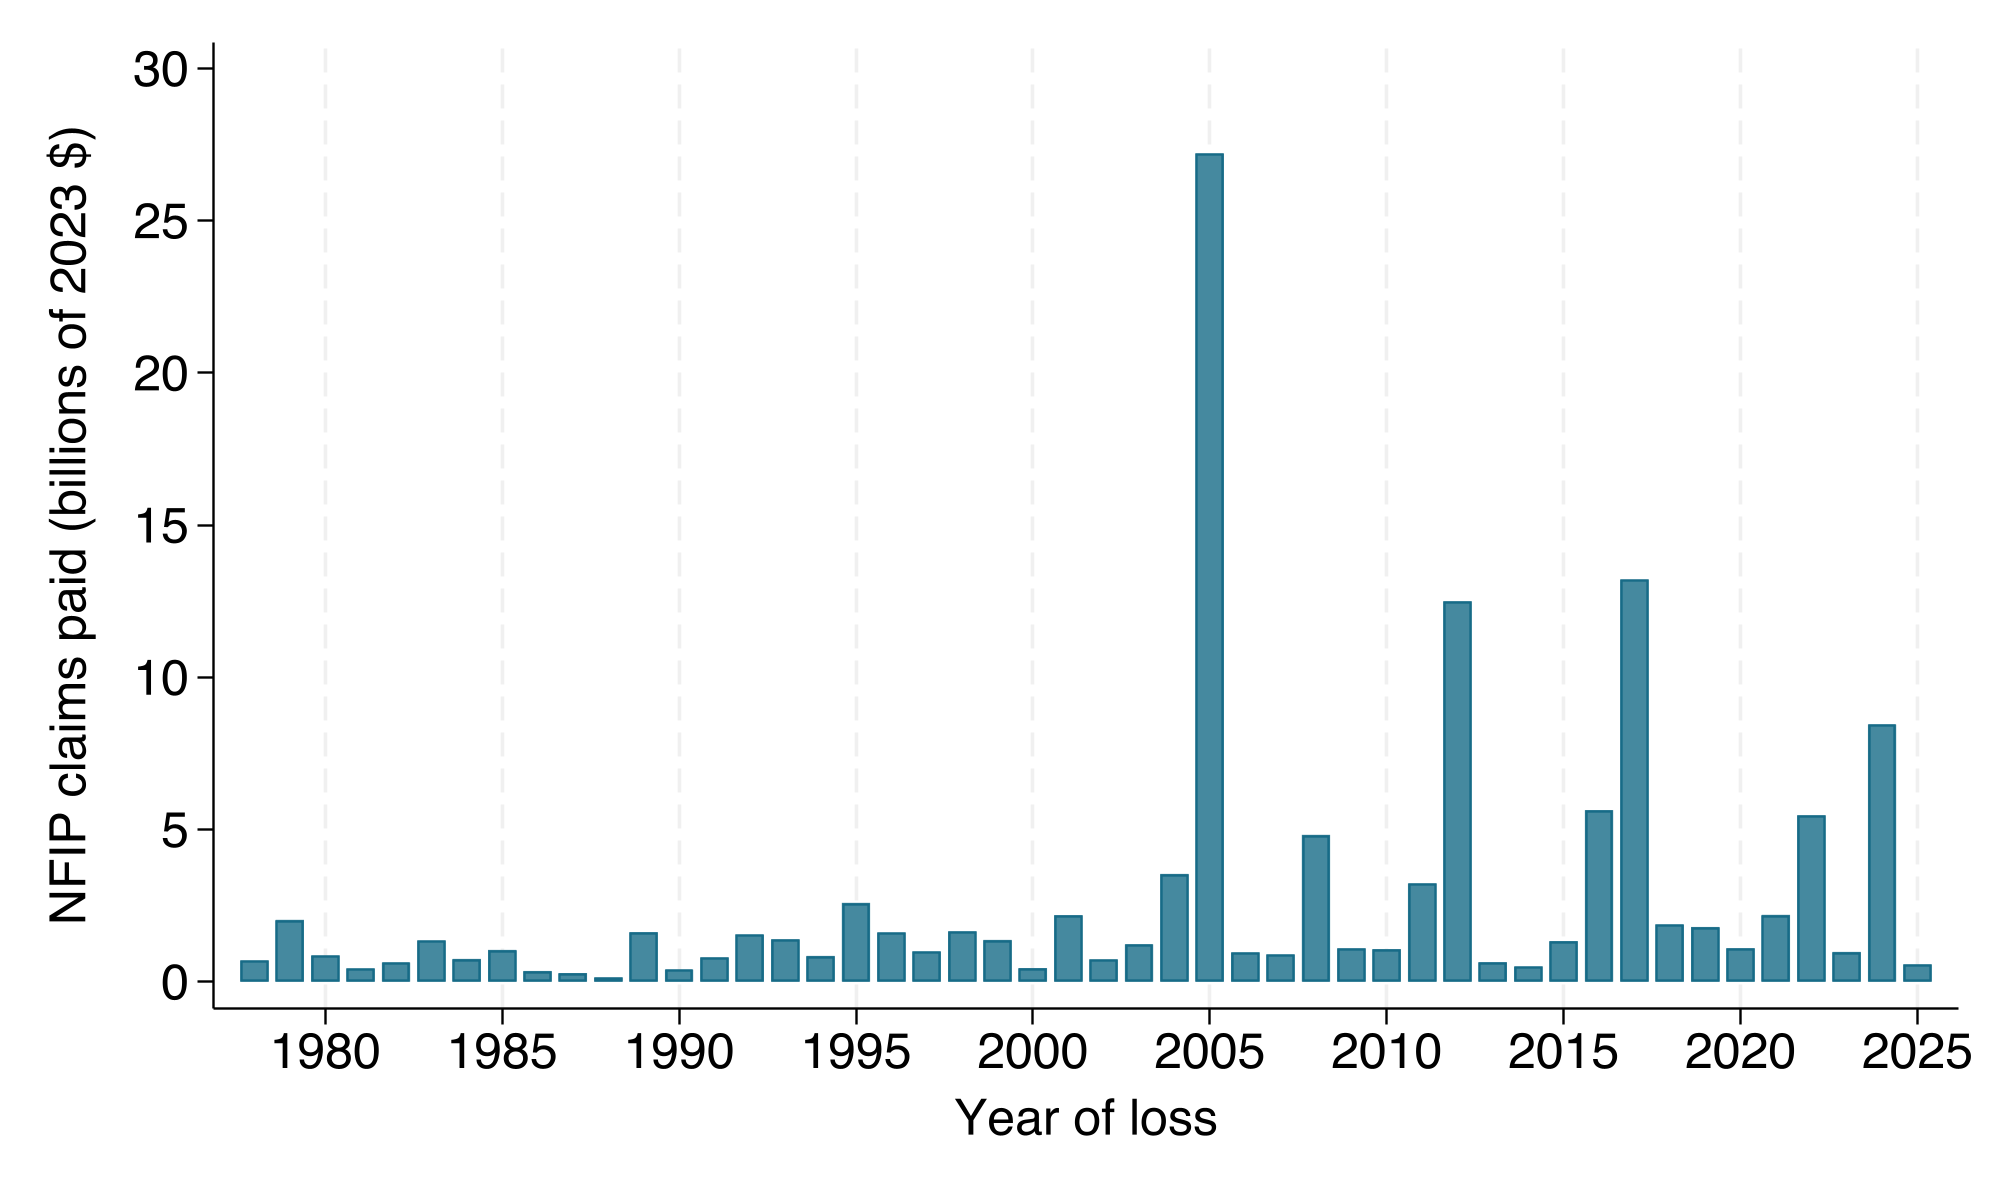
\includegraphics[width=0.70\textwidth]{nfip_claims_by_year.png}\\[2pt]
{\footnotesize Source: OpenFEMA NFIP redacted claims, all policies, by year of loss, 2023 dollars.}
\end{frame}

% Q: the policy count and coverage. Tabulated 09-22 on the raw national OpenFEMA v2 policy file
% (descriptives/scratch/nfip_policies_coverage.py, run on the other laptop; output/tables/
% nfip_policies_coverage_2025.xlsx): policies with a 2025 effective date, policyCount summed,
% building + contents coverage, all states and territories: 4.66 million policies (3.57 million
% records), $1.29 trillion coverage ($1.05 trillion building). FL LA TX are 2.83 million policies
% (61%) and $786 bn (61%). For comparison FEMA reports 4.7 million policies in force and $1.28
% trillion (Watermark, FY2022 Q4); 4.55 million policies in May 2026 (CRS IN10835). The v2 dataset
% is frozen at 06-01-2026 and deprecated on 10-15-2026 in favour of v3.
% Q: the "50% below cost" number. Verified 09-21 against the NBER WP 35408 PDF. It is Gruber and
% Solomon's own calculation on their FOIA policy panel (3,529,254 NFIP policies priced under RR2.0,
% nationwide, all flood zones): mean billed premium before RR2.0 $944 vs mean RR2.0 full-risk premium
% $1,739 (their Table 4), i.e. the average policy paid 54% of full risk, "approximately a 50% subsidy"
% (pp. 7-8, 26 and fn. 26). So it is ALL policies, not SFHA only; inside the SFHA the pre-FIRM
% discount was larger, outside it the community-rating "twist" made low-risk policies pay relatively
% more. Their "more than 50% lower than expected costs (CBO 2017)" on p. 3 does not match CBO's own
% summary: CBO found premiums $1.4bn short of expected costs on 5 million policies (a shortfall of
% roughly a quarter of premium income, concentrated in coastal counties), so CBO is not a source
% for the 50% figure and is no longer cited on the slide.
\begin{frame}{Setting}
\textbf{Insurance:} National Flood Insurance Program (NFIP)
\begin{itemize}
    \item Primary insurer against flood risk in the U.S.
    \begin{itemize}
        \item 4.7 million policies and \$1.3 trillion in coverage in 2025; the largest natural disaster insurance program in the world
    \end{itemize}
    \item Premiums held below risk by statute, on affordability grounds: before Risk Rating 2.0 the average policy paid about half its full-risk premium (Gruber \& Solomon 2026)
    \item Ongoing reform is moving premiums toward risk
\end{itemize}
\textbf{Adaptation:} Home elevations
\begin{itemize}
    \item Primary property-level protection against flood risk
    \item Mandatory for new construction in high-risk zones
    \item Retrofitting an existing house is effective but costly: median declared permit cost \$146{,}000; FEMA grant projects \$160{,}000--225{,}000 per home
\end{itemize}
\end{frame}

\begin{frame}{Research Question}
\begin{itemize}
    \item \textbf{Question:} A public insurer can subsidize premiums or adaptation investment. What is the optimal policy design?
    \item \textbf{Key forces:}
    \begin{itemize}
        \item Premium subsidies keep insurance affordable but mute the return to investment
        \item Risk-based pricing restores the incentive but pushes households out of coverage
        \item Investment subsidies keep households insured and lower claims directly
    \end{itemize}
    \item \textbf{This paper:} joint model of insurance take-up and investment, estimated on NFIP microdata
\end{itemize}
\end{frame}

\begin{frame}{Related Literature}
\textbf{1. Subsidized disaster insurance and adaptation}
\begin{itemize}
    \item Low willingness to pay; houses built under elevation mandates less likely to insure (Wagner 2022; Hovekamp \& Wagner 2023)
    \item Premium subsidies remain optimal once the spillover onto disaster aid is accounted for (Gruber \& Solomon 2026)
    \item Subsidies slow long-run adaptation; targeting restores it (Obolensky 2024)
\end{itemize}
\textbf{2. Preventive care in health insurance}
\begin{itemize}
    \item Insurers should cover prevention when the insured ignore its effect on premiums (Ellis \& Manning 2007; Newhouse 2006)
    \item Cost-sharing on upstream care raises downstream claims, often paid by another payer (Chandra, Gruber \& McKnight 2010; Starc \& Town 2018)
    \item Root: market insurance and self-protection as complements (Ehrlich \& Becker 1972)
\end{itemize}
\end{frame}

\begin{frame}{Related Literature (Continued)}
\small
\textbf{3. The disaster insurance puzzle: why is take-up so low?}
\begin{itemize}
    \item Flood insurance coverage surprisingly low (Kunreuther \& Pauly 2004; Wagner 2022)
    \item Risk misperception and salience explain take-up patterns (Gallagher 2014; Kousky 2010; Xu \& Box-Couillard 2024)
\end{itemize}
\textbf{4. Ex ante insurance vs.\ ex post aid (Samaritan's dilemma)}
\begin{itemize}
    \item Expected relief crowds out insurance demand for floods (Raschky et al.\ 2013; Kousky et al.\ 2018; Gruber \& Solomon 2026) and crops (Deryugina \& Kirwan 2018; Philippi \& Schiller 2024)
\end{itemize}
\textbf{5. Moral hazard in natural disaster insurance markets}
\begin{itemize}
    \item Location margin: insurance stimulates development and migration (Fabian 2024; Peralta \& Scott 2024; Browne et al.\ 2019)
    \item Mitigation margin: small effects of insurance prices on risk reduction (Hudson et al.\ 2017; Kousky 2019; Gruber \& Solomon 2026)
\end{itemize}
\end{frame}

% =============================================================================
\section{Background}
% =============================================================================

\begin{frame}{The National Flood Insurance Program}
\begin{itemize}
    \item \textbf{FEMA-administered, federally backed:} over 90\% of U.S. residential flood policies; cumulative claims have left the program \$20.5 billion in debt to the Treasury
    \item \textbf{Flood Insurance Rate Maps (FIRMs)} define flood zones and the Base Flood Elevation (BFE)
    \begin{itemize}
        \item Post-FIRM construction in high-risk zones (SFHAs) must be elevated above the BFE
        \item Pre-FIRM homes are exempt from elevation requirements and were charged heavily subsidized premiums
    \end{itemize}
    \item \textbf{Pricing reforms:}
    \begin{itemize}
        \item \textbf{Biggert-Waters (2012) / HFIAA (2014):} phase out pre-FIRM subsidies
        \item \textbf{Risk Rating 2.0 (2021--23):} replaces zone-based rating with property-level full-risk premiums
        \item Under both, subsidized policies converge to full-risk prices along a glide path of 5--18\% annual increases
    \end{itemize}
\end{itemize}
\end{frame}

% Counts from clean/hma_elevation.dta (funded projects only: approved, obligated or closed), all
% single-family elevation records: HMGP 8,868 properties, FMA + SRL 5,268, other programs 334.
% Dollars are the federal share summed once per project, 2023 $: HMGP $2.21bn, FMA + SRL $1.04bn.
% The "3% of 181,000 repetitive-loss properties" line is unchanged from the 09-08 draft.
\begin{frame}{Home Elevations}
\begin{itemize}
    \item \textbf{Cheap ex ante, expensive ex post.} Building a new house a foot higher adds about 0.25--1.5\% to construction cost; lifting an existing house costs \$150{,}000--225{,}000
    \item \textbf{What drives retrofit cost:} lifting the slab foundation, the size and weight of the house, and how high it has to go
    \item \textbf{FEMA elevation grants} (Hazard Mitigation Assistance):
    \begin{itemize}
        \item \textbf{HMGP}: post-disaster, administered by the state emergency agency; about 8{,}900 single-family elevations and \$2.2 billion since 1993
        \item \textbf{FMA}: financed out of NFIP premiums, targets repetitive-loss homes; about 5{,}300 elevations and \$1.0 billion since 1997, roughly 200 homes a year
    \end{itemize}
    \item \textbf{Elevations are modest:} in the past 20 years FMA has elevated about 3\% of roughly 181{,}000 repetitive-loss properties on NFIP's list
\end{itemize}
\end{frame}

% =============================================================================
\section{Data}
% =============================================================================

\begin{frame}[label=data_sources]{Data Sources}
\textbf{Sample}: NFIP-insured single-family homes in SFHAs, Florida, Louisiana, Texas, 2009--2025
\begin{itemize}
    \item \textbf{NFIP.} Universe of policy transactions, plus the claims and multiple-loss files
    \begin{itemize}
        \item Premiums, coverage, flood zone, post-FIRM status, RL/SRL status, claims by year
        \item Addresses are redacted: properties identified by construction date, block group, and policy origination date
    \end{itemize}
    \item \textbf{FEMA HMA.} Elevation grants: program (FMA vs.\ HMGP), cost, and number of properties, merged at the county
    \item \textbf{Builty permits.} Building permits from municipal feeds \hyperlink{builty_appendix}{\beamergotobutton{Appendix}}
    \begin{itemize}
        \item Elevations identified from permit text; retrofits separated from elevated new construction; declared project value
    \end{itemize}
    \item \textbf{ATTOM tax assessor.} Property-year market value and characteristics; carries the address that links permits to NFIP
    \item \textbf{NFHL flood maps.} FEMA flood zone for ATTOM properties
\end{itemize}
\end{frame}

% Figure: descriptives/scratch/elevations_by_state.do -> output/figures/elevations_by_state.png.
% Q: raw counts, not the analysis sample. Each bar counts properties in its own source file
% across all 20 states: Builty retrofit permits from the per-state clean files, HMA from the
% clean grant file, NFIP flag flips from the 20-state panel. The funding correction from GitHub
% (issue #13) is applied: HMA counts only approved, obligated or closed projects (LA 5,658 vs
% 7,400 raw; TX 1,090 vs 1,532; FL 436 vs 1,043). The like-for-like rate on the analysis sample
% is in output/tables/elevations_by_state.xlsx and quoted in the bullet.
\begin{frame}{Why These Three States}
\begin{columns}[T,onlytextwidth]
    \begin{column}{0.66\textwidth}
        \centering
        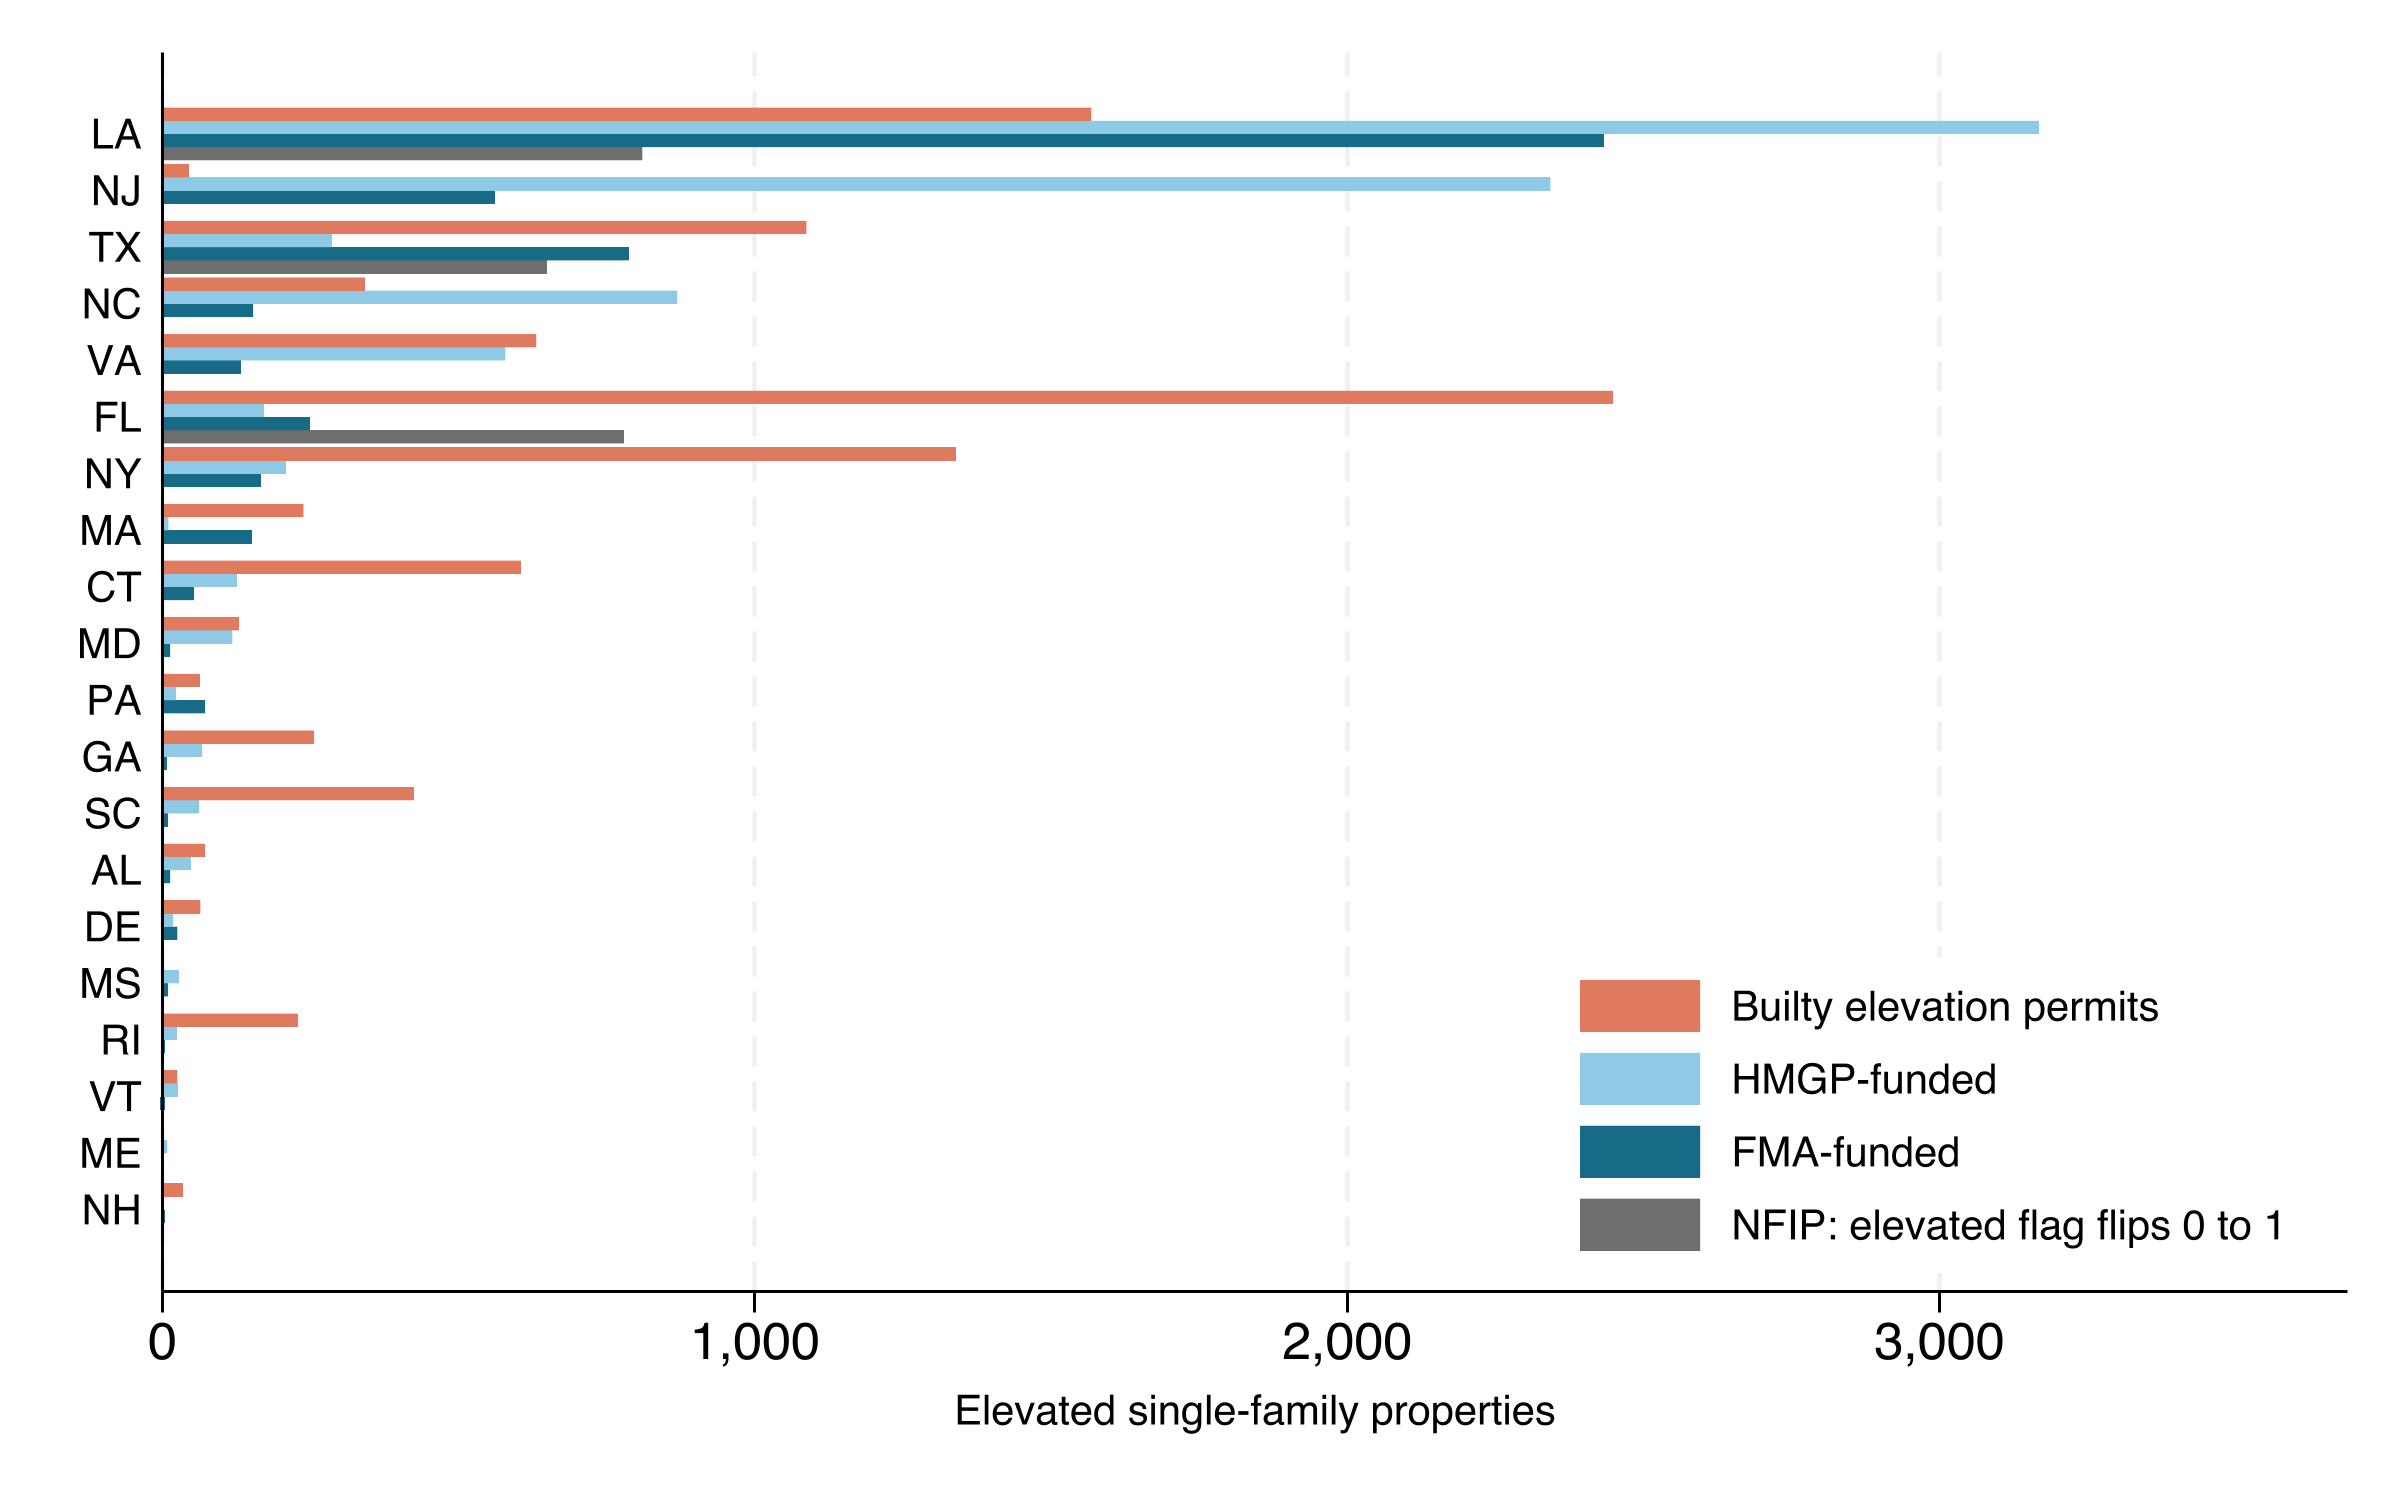
\includegraphics[width=\linewidth]{elevations_by_state.png}
    \end{column}
    \begin{column}{0.32\textwidth}
        \begin{itemize}
            \item Counts by source across 20 states; HMA counts funded projects only
            \item Louisiana is large on both the permit and the grant side; Florida has the most permits; Texas is in between
            \item On the analysis sample: 3.0 (LA), 2.3 (TX) and 1.1 (FL) elevation events per 1{,}000 insured SFHA homes
        \end{itemize}
    \end{column}
\end{columns}
\end{frame}

% Table: descriptives/summary_table.do (master.do switch) -> output/tables/summary_table.xlsx.
% Premium, loss ratio and the claim share are over property-years; the rest over properties
% (cumulative claims at the last policy year). "Elevated ex ante" = flagged elevated in the
% first policy year with no in-sample event; "Elevation retrofit" = the harmonized event
% (Builty permit, NFIP flag flip, or ICC payment with continued coverage). Retrofit cost is the
% Builty declared value (FL and TX permits). Property value is the ATTOM market value.
\begin{frame}{Summary Statistics}
\vspace{-.5cm}
\begin{table}\centering\small
\textbf{NFIP-insured single-family properties in SFHAs, FL LA TX, 2009--2025}
\vspace{2mm}
\begin{tabular}{lrrr}
\toprule
 & All & Pre-FIRM & Post-FIRM \\
\midrule
\quad Annual premium, median (\$)            & 644       & 888       & 574       \\
\addlinespace
\quad Claims paid / premiums collected       & 1.07      & 1.26      & 0.82      \\
\quad Any claim in a year (share)            & 0.012     & 0.016     & 0.008     \\
\quad Cumulative claims, median (\$) \\
\quad\quad among claimants                   & 82{,}600  & 96{,}500  & 45{,}900  \\
\quad\quad among repetitive loss             & 104{,}400 & 112{,}800 & 72{,}500  \\
\quad\quad among severe repetitive loss      & 122{,}300 & 124{,}600 & 98{,}200  \\
\addlinespace
\quad Property value, median (\$)            & 242{,}300 & 220{,}900 & 261{,}300 \\
\addlinespace
\quad Elevated ex ante                       & 450{,}281 & 173{,}018 & 277{,}263 \\
\quad Elevation retrofit                     & 4{,}993   & 3{,}543   & 1{,}450   \\
\quad Retrofit cost, median (\$)             & 145{,}900 & 159{,}000 & 43{,}000  \\
\midrule
Number of properties                         & 3{,}291{,}652 & 1{,}621{,}829 & 1{,}669{,}823 \\
\bottomrule
\end{tabular}
\end{table}
\end{frame}

% Figures: descriptives/histograms.do -> output/figures/{elevation_cost,claims}_histogram.png.
% Q: yes, both histograms (and the scatter on the next frame) are computed from analysis.dta,
% one row per property: cumulative claims at the last policy year among claimants; Builty
% declared cost among permitted homes; both with a $1k display floor.
\begin{frame}{Elevation Costs vs.\ Cumulative Claims}
\begin{columns}[T,onlytextwidth]
    \begin{column}{0.46\textwidth}
        \centering
        \textbf{Elevation cost}
        \vspace{0.2em}
        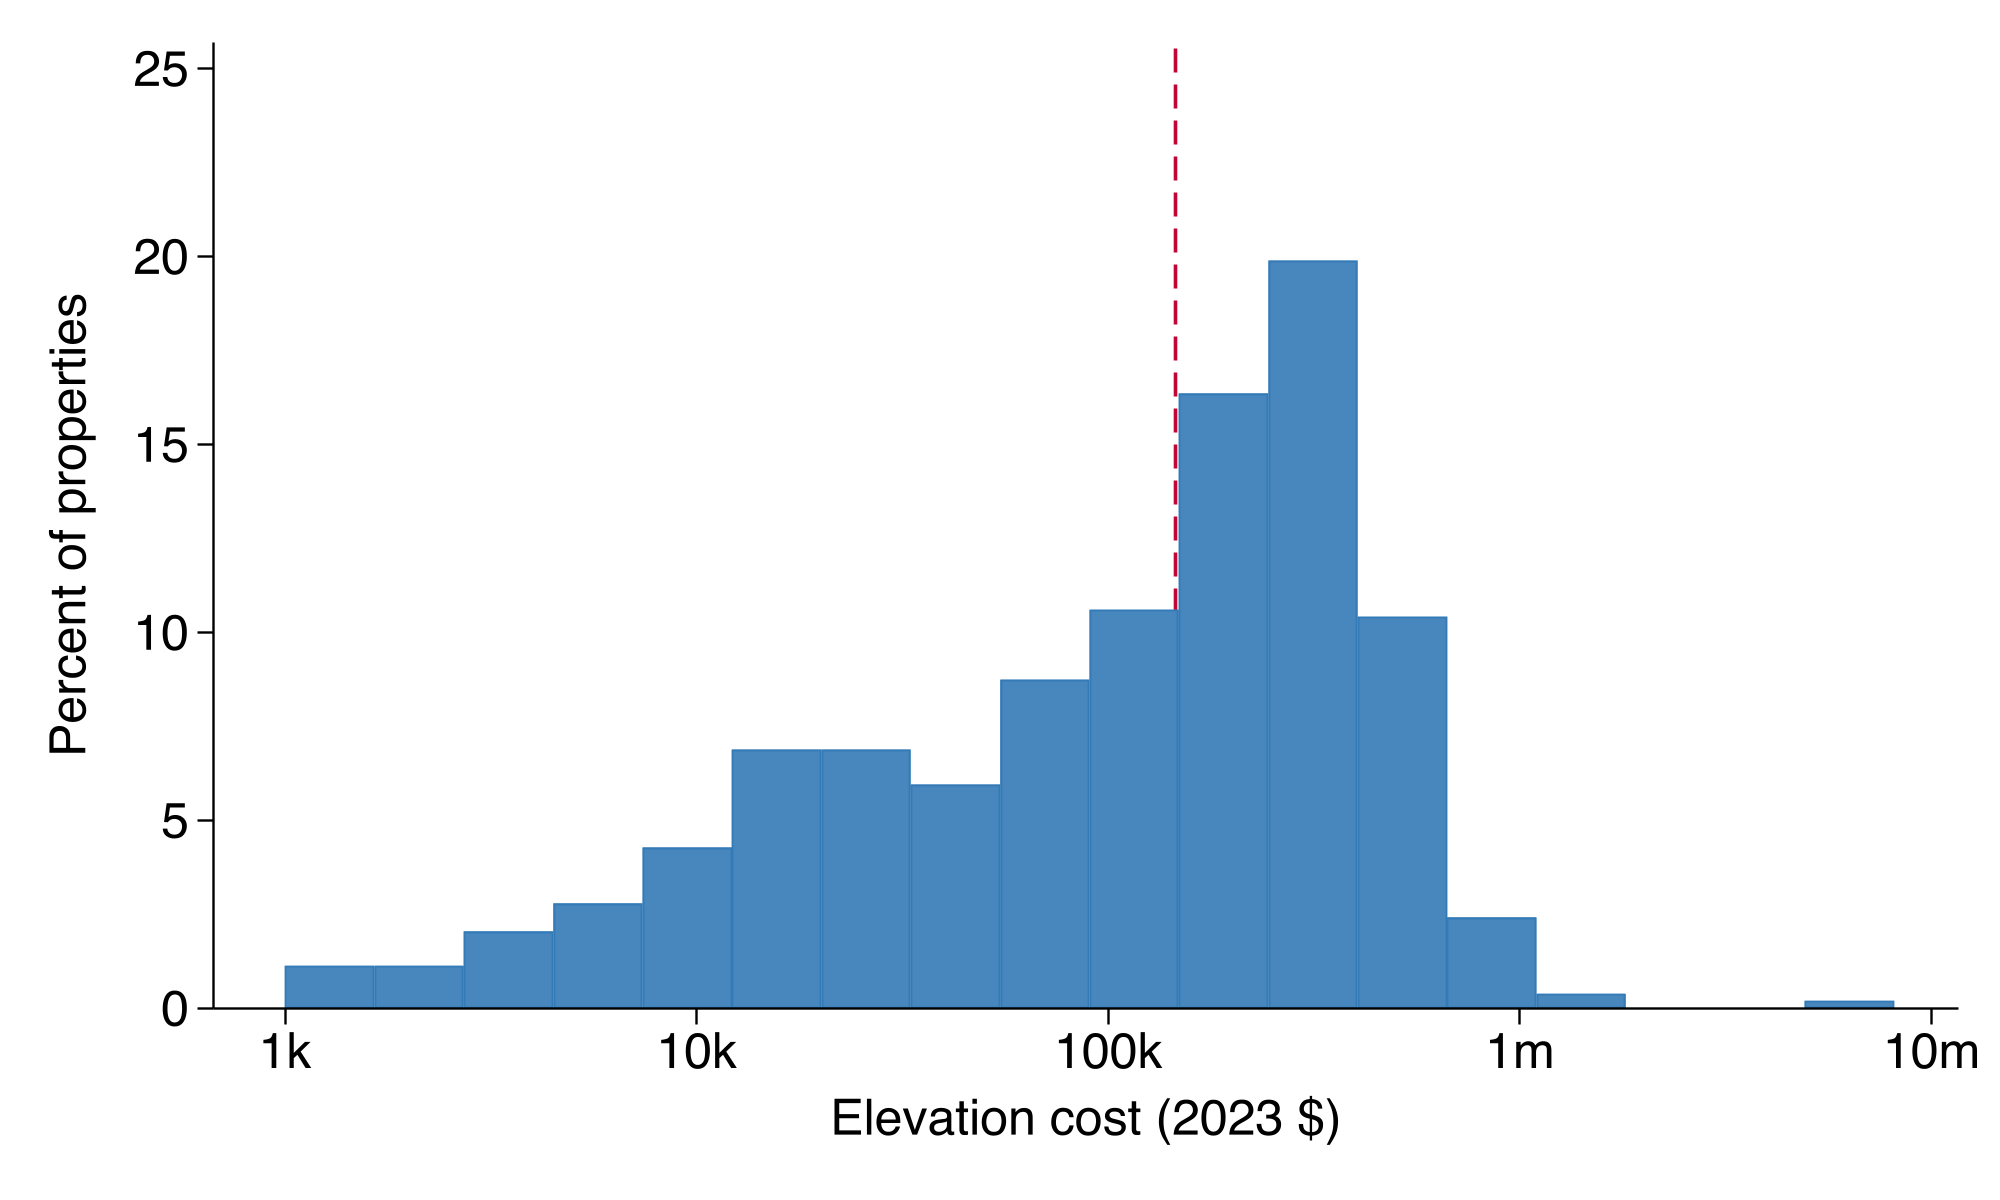
\includegraphics[width=\linewidth]{elevation_cost_histogram.png}
    \end{column}
    \begin{column}{0.46\textwidth}
        \centering
        \textbf{Cumulative NFIP claims}
        \vspace{0.2em}
        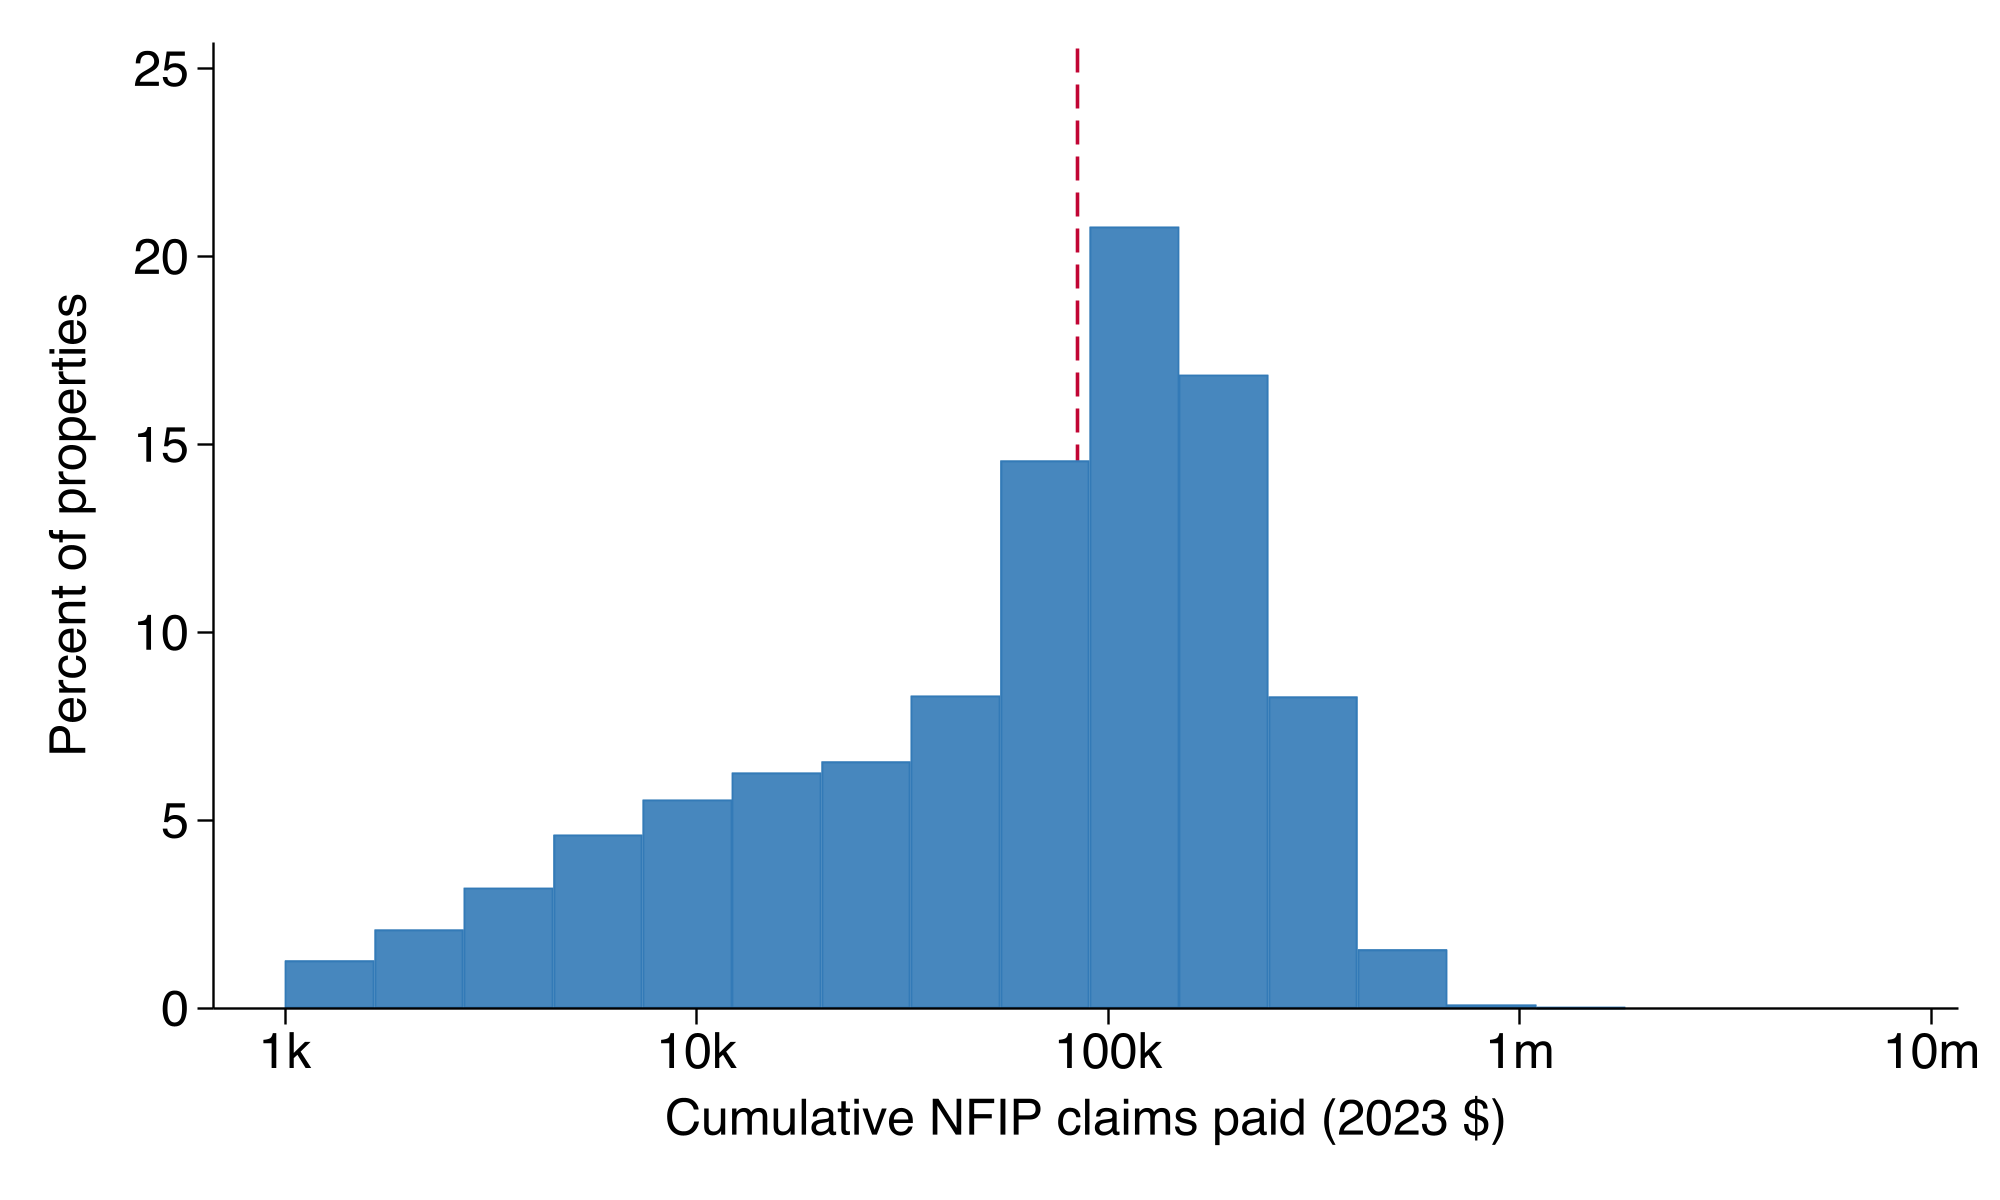
\includegraphics[width=\linewidth]{claims_histogram.png}
    \end{column}
\end{columns}
\begin{itemize}
    \item The two distributions overlap: for many claimants, the claims already paid are of the order of an elevation
    \item Wide dispersion on both sides, so the return to elevating differs a lot across homes
\end{itemize}
\end{frame}

% Figure: descriptives/histograms.do -> output/figures/claims_vs_elevation_cost.png. Each point
% is a permitted home with a declared cost and at least $1k of claims paid before the permit;
% homes without prior claims are not shown. Keep this or the histogram frame, not both.
\begin{frame}{Elevation Cost Against Claims Paid Before the Permit}
\begin{columns}[T,onlytextwidth]
    \begin{column}{0.55\textwidth}
        \centering
        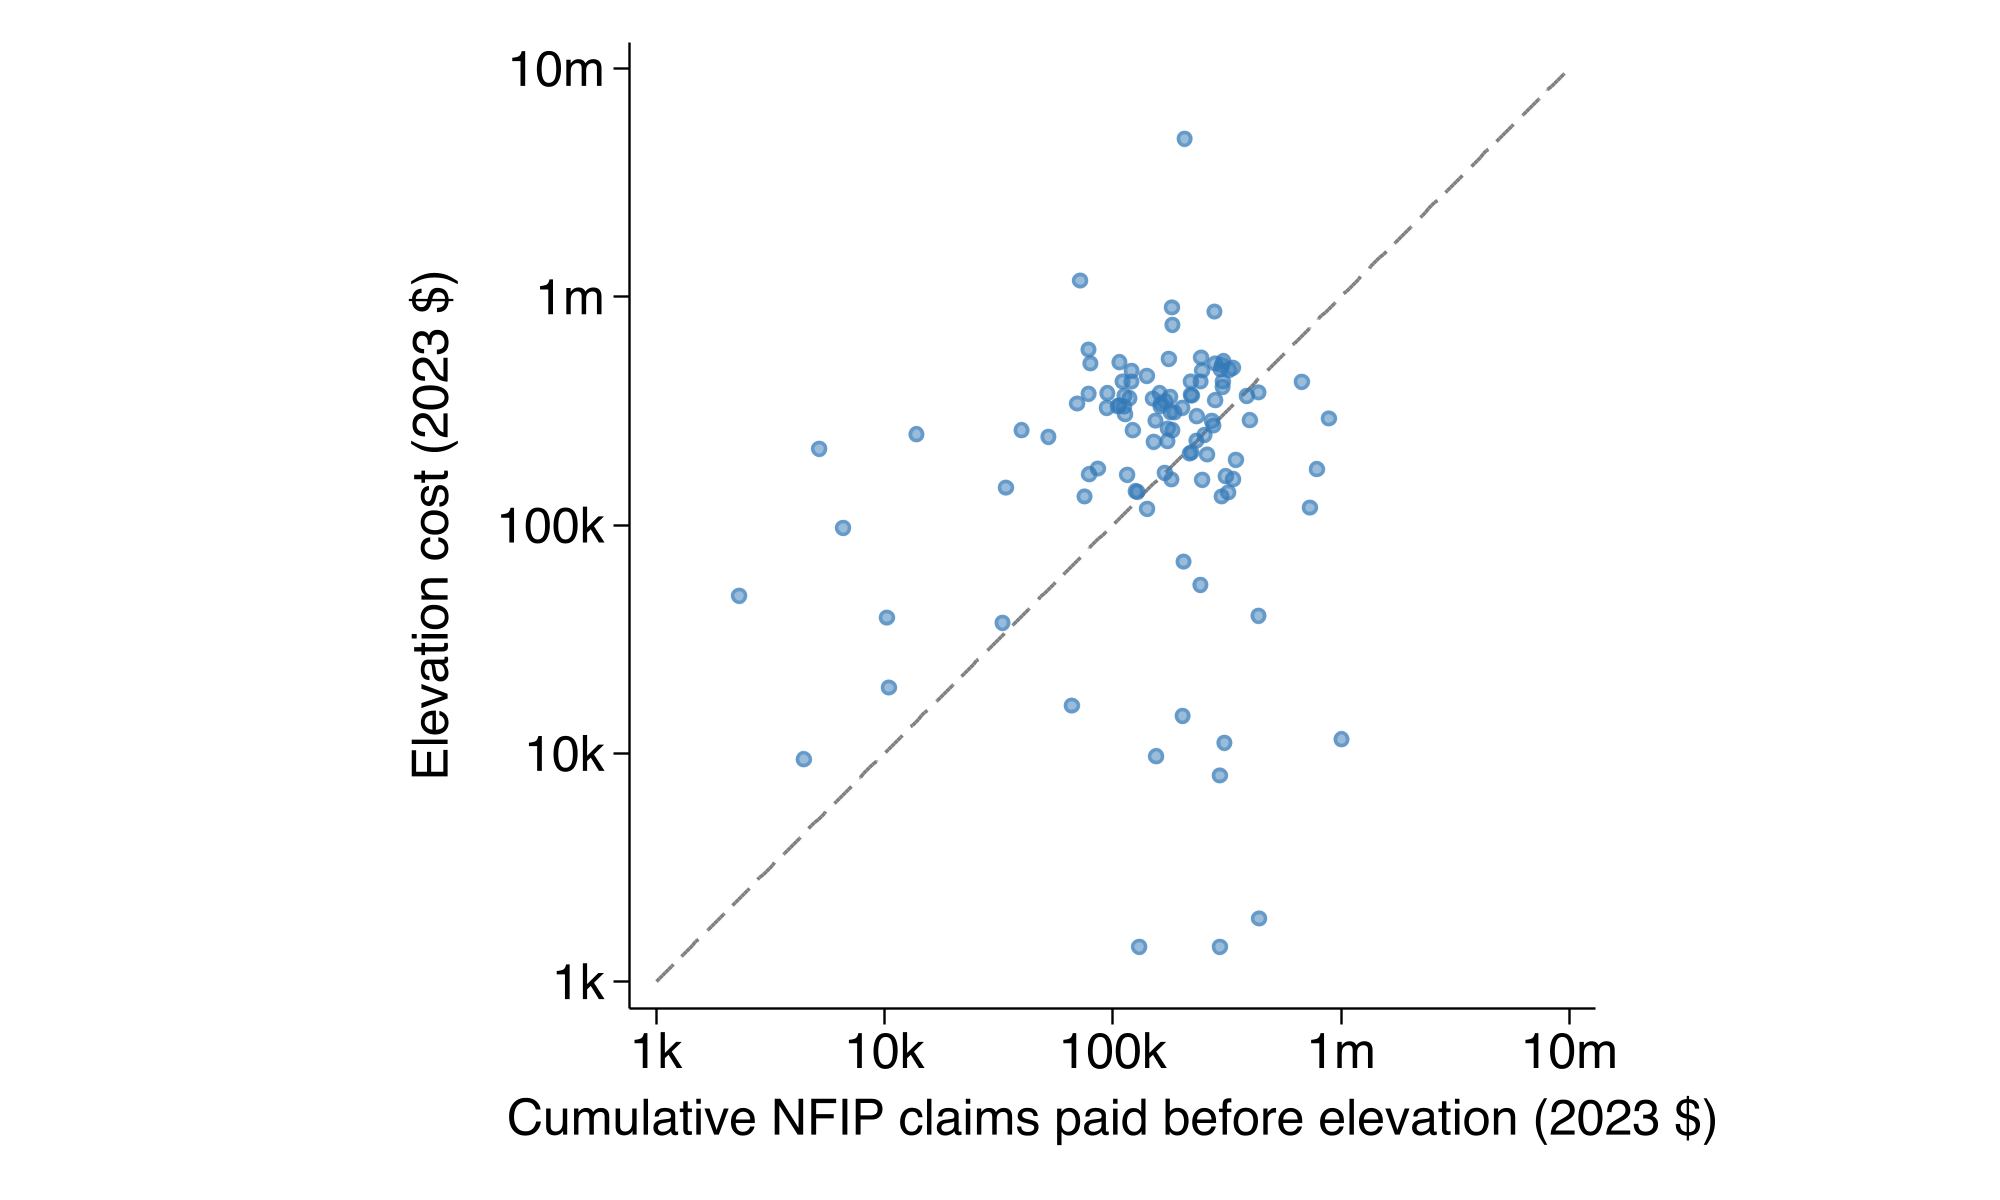
\includegraphics[width=0.9\linewidth]{claims_vs_elevation_cost.png}
    \end{column}
    \begin{column}{0.43\textwidth}
        \begin{itemize}
            \item One point per elevated home with a declared cost and prior claims
            \item Below the 45-degree line, the claims already paid exceed the cost of elevating
            \item Most homes elevate at a cost several times their prior claims; for a minority, one flood had already cost more than the elevation
        \end{itemize}
    \end{column}
\end{columns}
\end{frame}

% =============================================================================
\section{Reduced-Form Evidence}
% =============================================================================

% Design and numbers match analysis/es_elevation.do (in master.do, switch es_elevation). The 09-22
% script pools every harmonized event (permit, NFIP flag flip, ICC payment) in sections 1-3 and
% then runs the same design by source in section 4; the deck's main results use the permit panels
% (es_elevation_{premium,claim}_permit.png), the same-flood comparison is its own permit-only
% script (analysis/same_flood_claims.do), and the pooled and by-source plots are in the appendix. Sample: 1,573 permitted homes in cohorts
% 2012-2022 (490 flip, 741 ICC set aside), 235,400 never-elevated control homes, 143 counties.
\begin{frame}{Event-Study Design}
\small
For home $i$ in county $c$, flood zone $z$, and policy year $t$, with an elevation permit in year $\tau_i$:
\begin{equation*}
    y_{it} \;=\; \sum_{\substack{k=-5 \\ k \neq -1}}^{5} \beta_k \,\mathbf{1}\{t - \tau_i = k\}
    \;+\; \alpha_i \;+\; \gamma_{czt} \;+\; \varepsilon_{it}
\end{equation*}
\begin{itemize}
    \item $y_{it}$: annual premium, or paid claim, in 2023 dollars
    \item $\alpha_i$: home fixed effect. $\gamma_{czt}$: county $\times$ flood zone (A/V) $\times$ year, which absorbs local floods and the move to risk-based pricing
    \item $\beta_k$: change relative to the year before the permit; endpoints binned at $\pm 5$. Each $\beta_k$ is the cohort-share-weighted average of cohort-specific coefficients (Sun \& Abraham 2021)
    \item Treated: homes with a Builty elevation permit in 2012--2022. Controls: homes never elevated by any source, so staggered permit timing does not contaminate $\beta_k$
    \item Standard errors clustered by county
\end{itemize}
\textbf{Identifying assumption:} absent the permit, outcomes of permitted homes would have moved in parallel with never-elevated homes in the same county, zone and year. Caveat: permits follow floods, so $k=-1$ is usually a flood year
\end{frame}

% Figure: es_elevation_premium_permit.png (es_elevation.xlsx, sheet event_study_permit).
% Post-permit coefficients t0..t+4 are +$3 to +$22 with SE $24-49; t+5 -$105 (SE 54).
\begin{frame}{Elevating Does Not Lower the Premium}
\centering
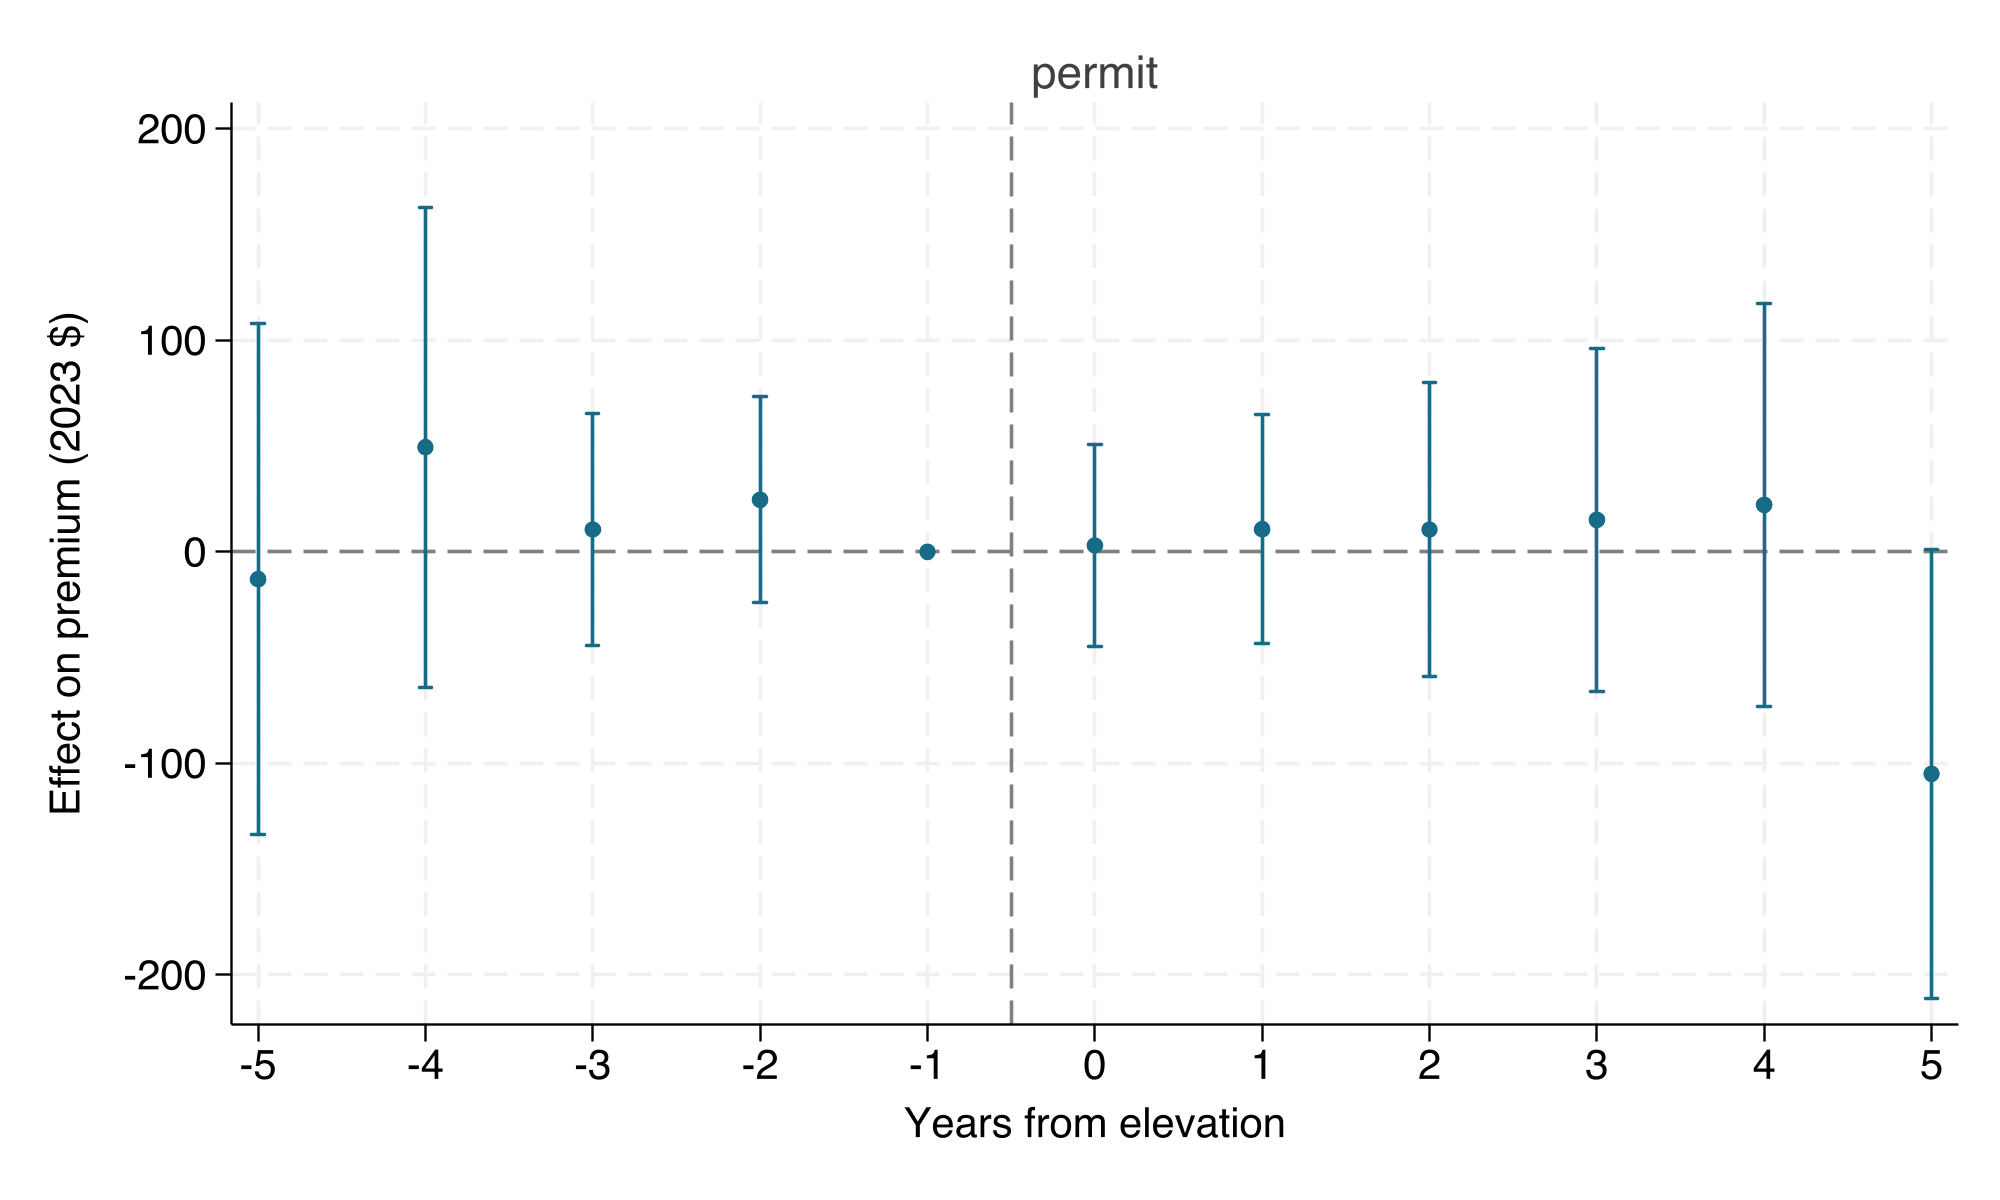
\includegraphics[width=0.60\textwidth]{es_elevation_premium_permit.png}
\begin{itemize}
    \item The insurer does not reward the investment: no drop in the premium in the five years after the permit
\end{itemize}
\end{frame}

\begin{frame}{Same-Flood Design}
\small
Floods are rare inside a five-year window, so effectiveness is measured on homes hit by the same flood: county-years in which at least 5\% of insured homes, and at least 50 homes, have a paid claim
\begin{equation*}
    y_{it} \;=\; \beta^{\text{pre}} \, \text{Pre}_{it} \;+\; \beta^{\text{post}} \, \text{Post}_{it}
    \;+\; \gamma_{czt} \;+\; \delta_{d(i) f(i)} \;+\; \varepsilon_{it}
\end{equation*}
\begin{itemize}
    \item $\text{Pre}_{it}$, $\text{Post}_{it}$: permitted home observed before, or after, its permit. Omitted group: never-elevated homes
    \item $\gamma_{czt}$: county $\times$ flood zone $\times$ year, so the comparison is within the same flood. $\delta_{df}$: construction decade $\times$ post-FIRM status
    \item $\beta^{\text{pre}}$ measures selection into elevation; $\beta^{\text{pre}} - \beta^{\text{post}}$ is the damage avoided per flood
    \item Standard errors clustered by county
\end{itemize}
\textbf{Identifying assumption:} within a flood, a permitted home's excess damage over its neighbors would have stayed at its pre-permit level without the elevation
\end{frame}

% Figure: analysis/same_flood_claims.do (master.do switch same_flood_claims) ->
% output/figures/same_flood_claims.png and output/tables/same_flood_claims.xlsx. Permit-only:
% 2,908 permitted homes, 206,939 never-elevated controls; 784 pre-permit and 527 post-permit
% home-years in flood county-years. Pre +$40,578 (SE 9,073), post -$727 (SE 2,089), difference
% $41,305 (SE 9,780). Raw means in flood years: never elevated $20.2k, permitted before $78.7k,
% permitted after $18.0k. Sheet npv: flood-year share 7.1%, $2,935 a year, 30 years at FEMA's 7%
% BCA rate (Hovekamp and Wagner use 80 years at 4%, which gives about $70k) = NPV $36,416,
% median declared permit cost $145,998, NPV/cost 0.25, payback 50 years. Run 09-22.
\begin{frame}{Elevating Lowers Claims}
\centering
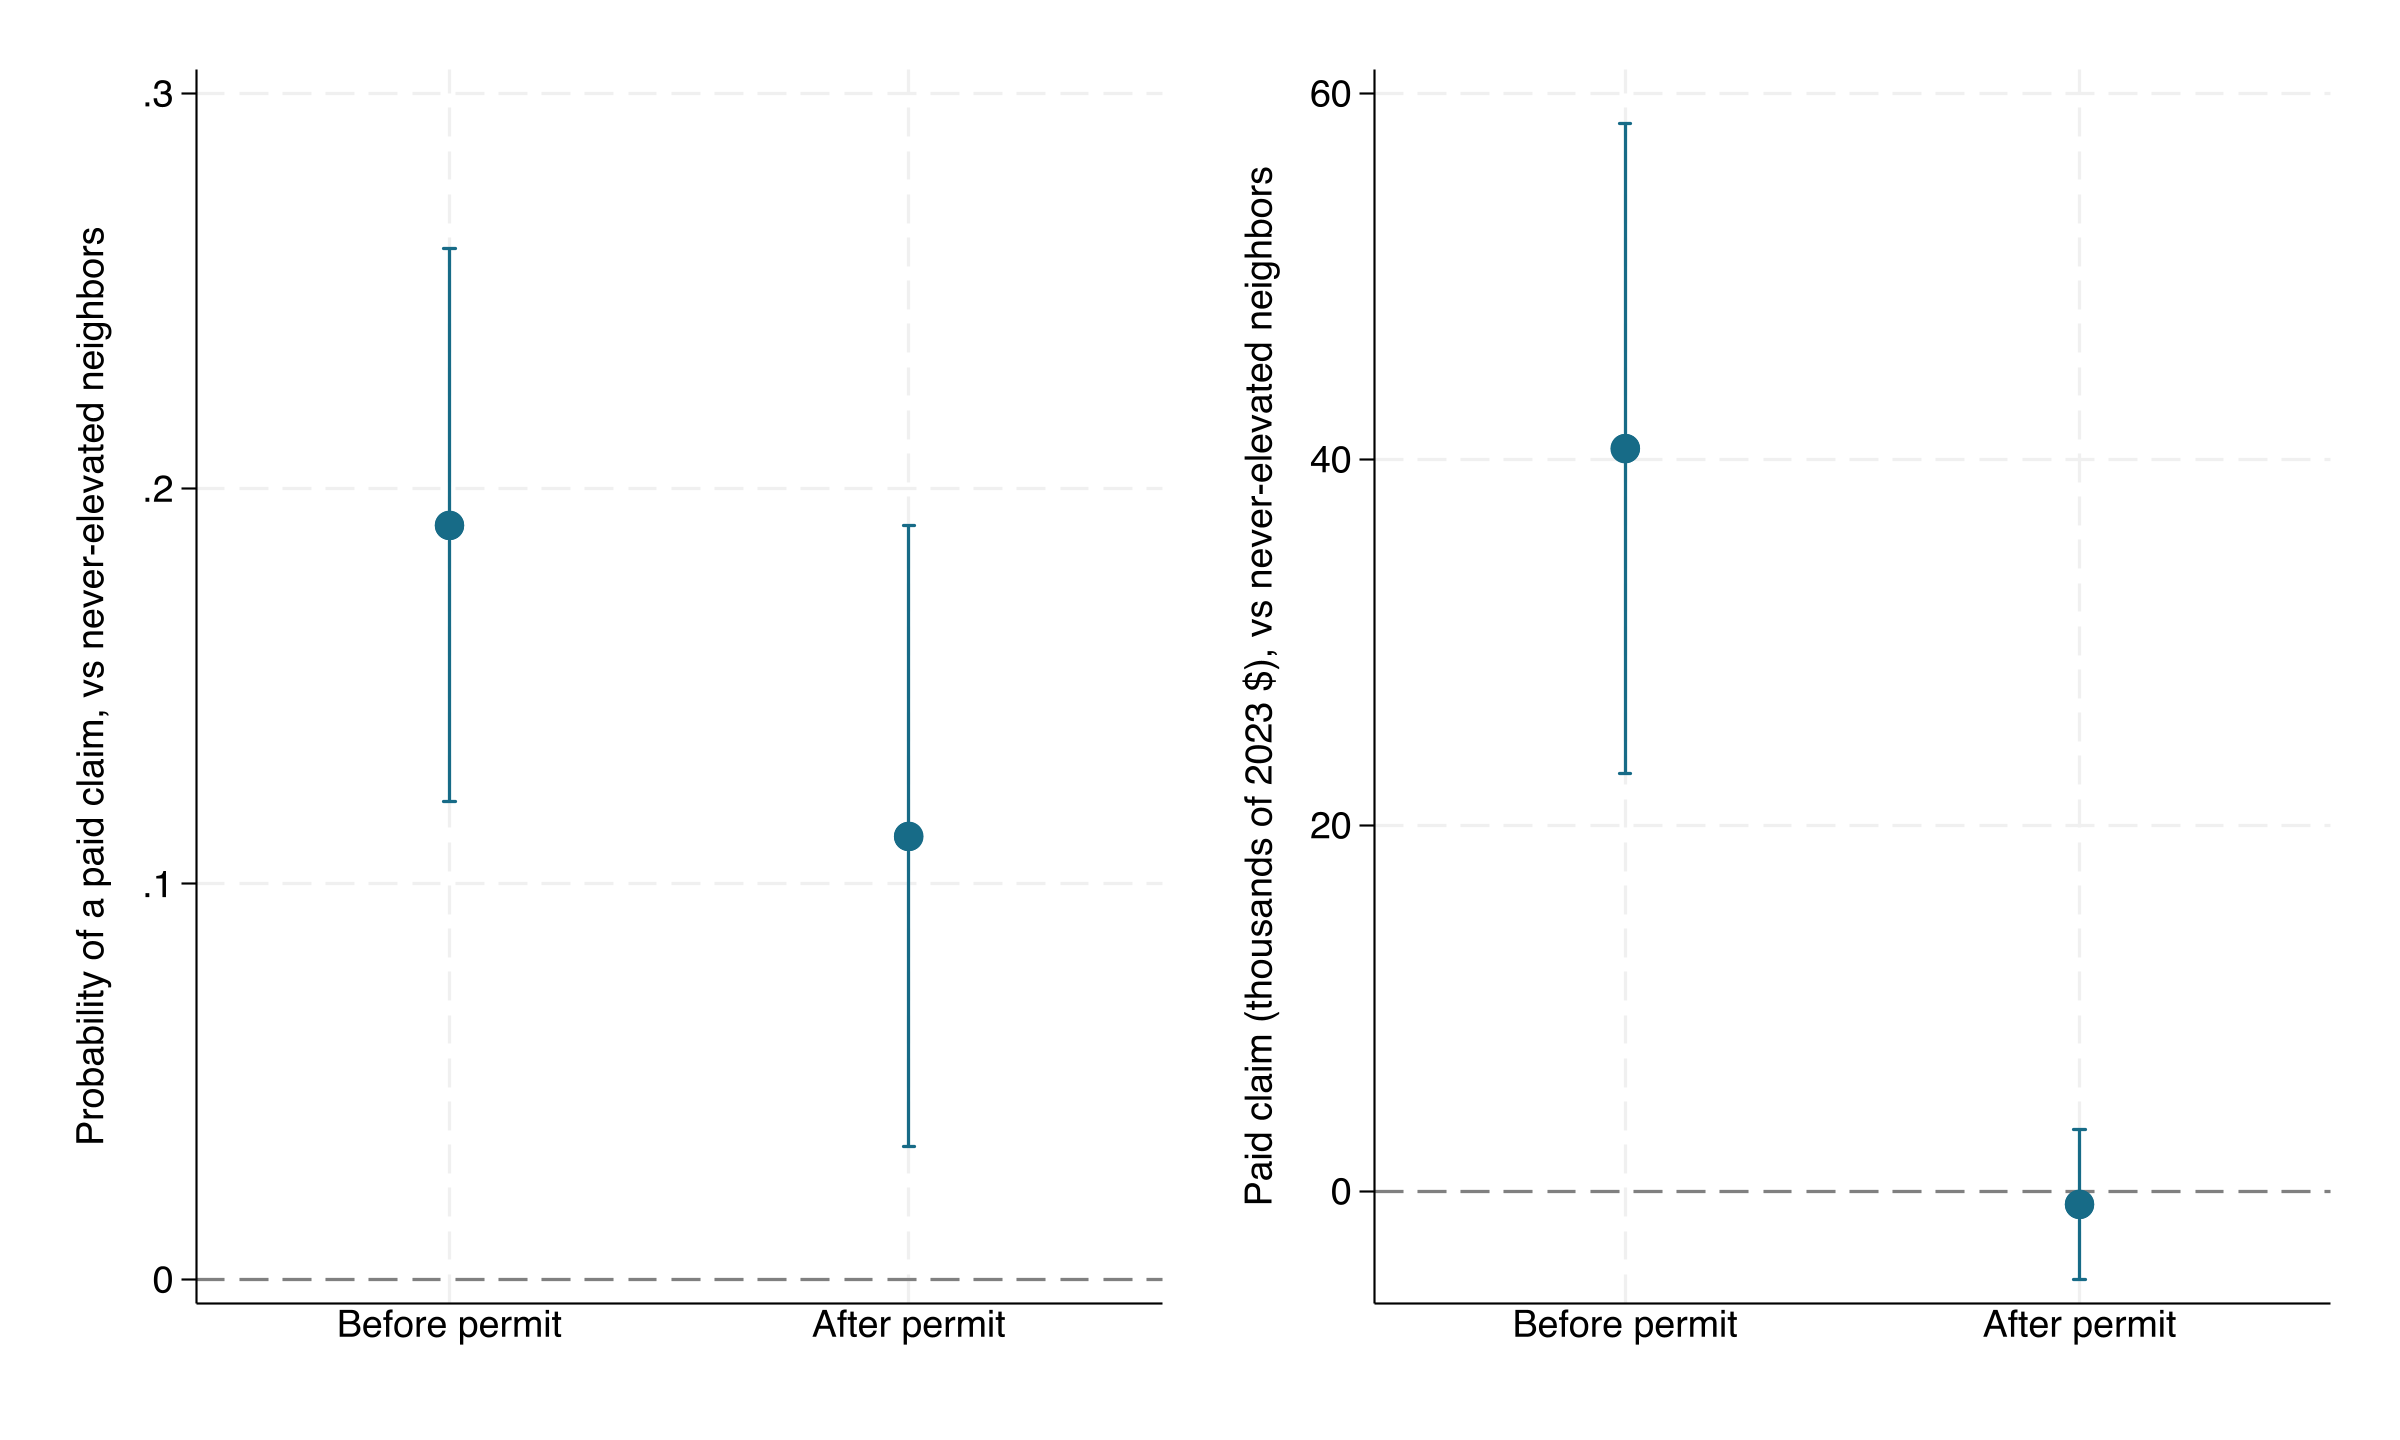
\includegraphics[width=0.58\textwidth]{same_flood_claims.png}
\begin{itemize}
    \item Same flood, same county and zone: homes that later elevate claim \$41k more than their neighbors before the permit, and the same as their neighbors after it
    \item \$41k per flood year $\times$ 7\% flood-year frequency $\approx$ \$2{,}900 a year; NPV over 30 years at 7\% $\approx$ \$36{,}000, a quarter of the median cost of \$146{,}000
\end{itemize}
\end{frame}

% =============================================================================
\section{Model \& Empirical Strategy}
% =============================================================================

\begin{frame}{Model}
\textbf{Joint model of insurance take-up and mitigation investment}
\begin{itemize}
    \item Household with house value $v$ and flood risk $\pi$ chooses whether to insure and whether to elevate
    \item Elevation cuts expected damage and, under risk-based pricing, the premium; it costs $(1-s)\,c$ plus a non-monetary cost $\kappa$ (time, disruption, the look of a raised house)
    \item Insurance pays capped claims at premium $p(E)$; uninsured losses are partly covered by ex post aid
    \item \textbf{Two policy instruments:} the premium schedule and the elevation subsidy $s$
    \item \textbf{Distortion:} subsidized premiums mute the return to elevating; risk-based premiums restore it but reduce take-up
    \item \textbf{Counterfactuals}, same government outlay: actuarially fair premiums vs.\ an elevation subsidy
\end{itemize}
\end{frame}

\begin{frame}{Estimation}
\begin{itemize}
    \item \textbf{Cost $c$:} Builty declared permit cost; HMA project cost per home
    \item \textbf{Response of investment to price:} FMA cost shares (75/90/100\%) and the elevation discount before vs.\ after Risk Rating 2.0
    \item \textbf{Effectiveness of elevation:} same-flood comparison above; literature (Hovekamp \& Wagner 2023; USACE 2021)
    \item \textbf{Insurance demand:} take-up response to the premium reforms below
    \item \textbf{Risk $\pi$:} claims history and flood zone
    \item \textbf{Non-monetary cost $\kappa$:} residual that matches observed elevation rates in FL, LA, TX
\end{itemize}
\end{frame}

\begin{frame}{Identifying Variation in Premiums}
Two NFIP pricing reforms generate house-level variation in premiums:
\begin{itemize}
    \item \textbf{Biggert-Waters (2012) / HFIAA (2014):} phase-out of historically subsidized premiums for pre-FIRM homes
    \begin{itemize}
        \item Exogenous price changes differentially affect \textbf{non-adapted} properties
        \hfill {\small\color{gray} Wagner (2022)}
    \end{itemize}
    \item \textbf{Risk Rating 2.0 (2021--):} property-level, risk-based pricing replaces the old rating system
    \begin{itemize}
        \item Within-property price increases toward a full-risk premium
        \hfill {\small\color{gray} Gruber and Solomon (2026)}
    \end{itemize}
\end{itemize}
\end{frame}

% =============================================================================
\section{Next Steps}
% =============================================================================

\begin{frame}{Next Steps}
\begin{itemize}
    \item \textbf{Data:} property-level grant records from Louisiana (GOHSEP, due end of October) and Rhode Island; ATTOM permit data as a replacement for Builty if the quote allows
    \item \textbf{Empirics:} elevation discount and take-up around Risk Rating 2.0; investment response to the FMA cost share
    \item \textbf{Model:} write down the household's elevation and insurance choice and what each moment pins down
\end{itemize}
\end{frame}

% =============================================================================
\appendix
\section{Appendix}
% =============================================================================

\begin{frame}[label=builty_appendix]{Builty Word Cloud \hyperlink{data_sources}{\beamerreturnbutton{Back to Data Sources}}}
\centering
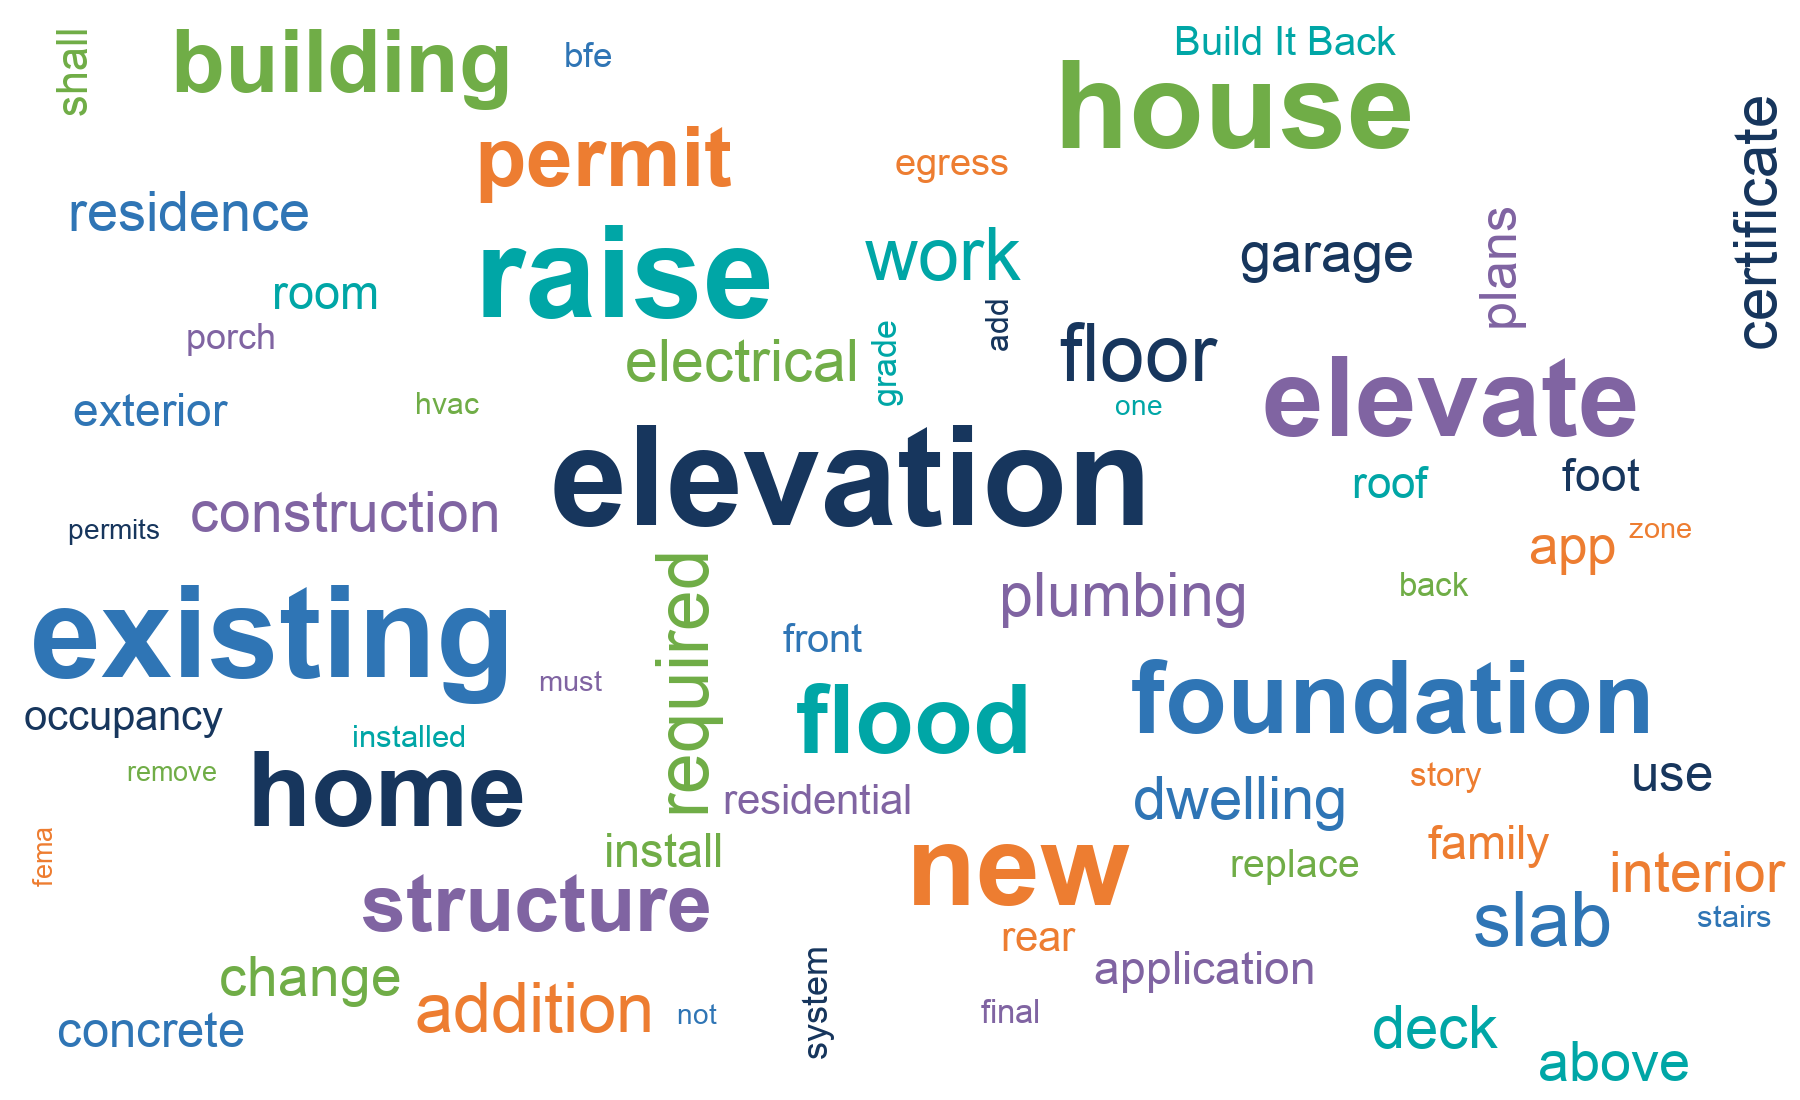
\includegraphics[width=0.8\linewidth]{builty_elevation_wordcloud.png}
\end{frame}

% Figures: es_elevation_{claim,premium}_by_source.png (section 4 of es_elevation.do). The three
% sources date three different moments: the permit is issued after the flood (flood at t-1),
% the ICC year is the year of loss (flood at t0 by construction, +$125k), and the flag flip is
% the insurer's re-rating after the work (no flood in the window, premium falls from t+1 with
% a downward pre-trend). Pooling them gives the +$46k spike at t0 and the -$140 to -$360
% premium drop of the pooled run; the permit panels alone carry the deck's results.
\begin{frame}{Appendix: Claims Around the Elevation, by Source}
\centering
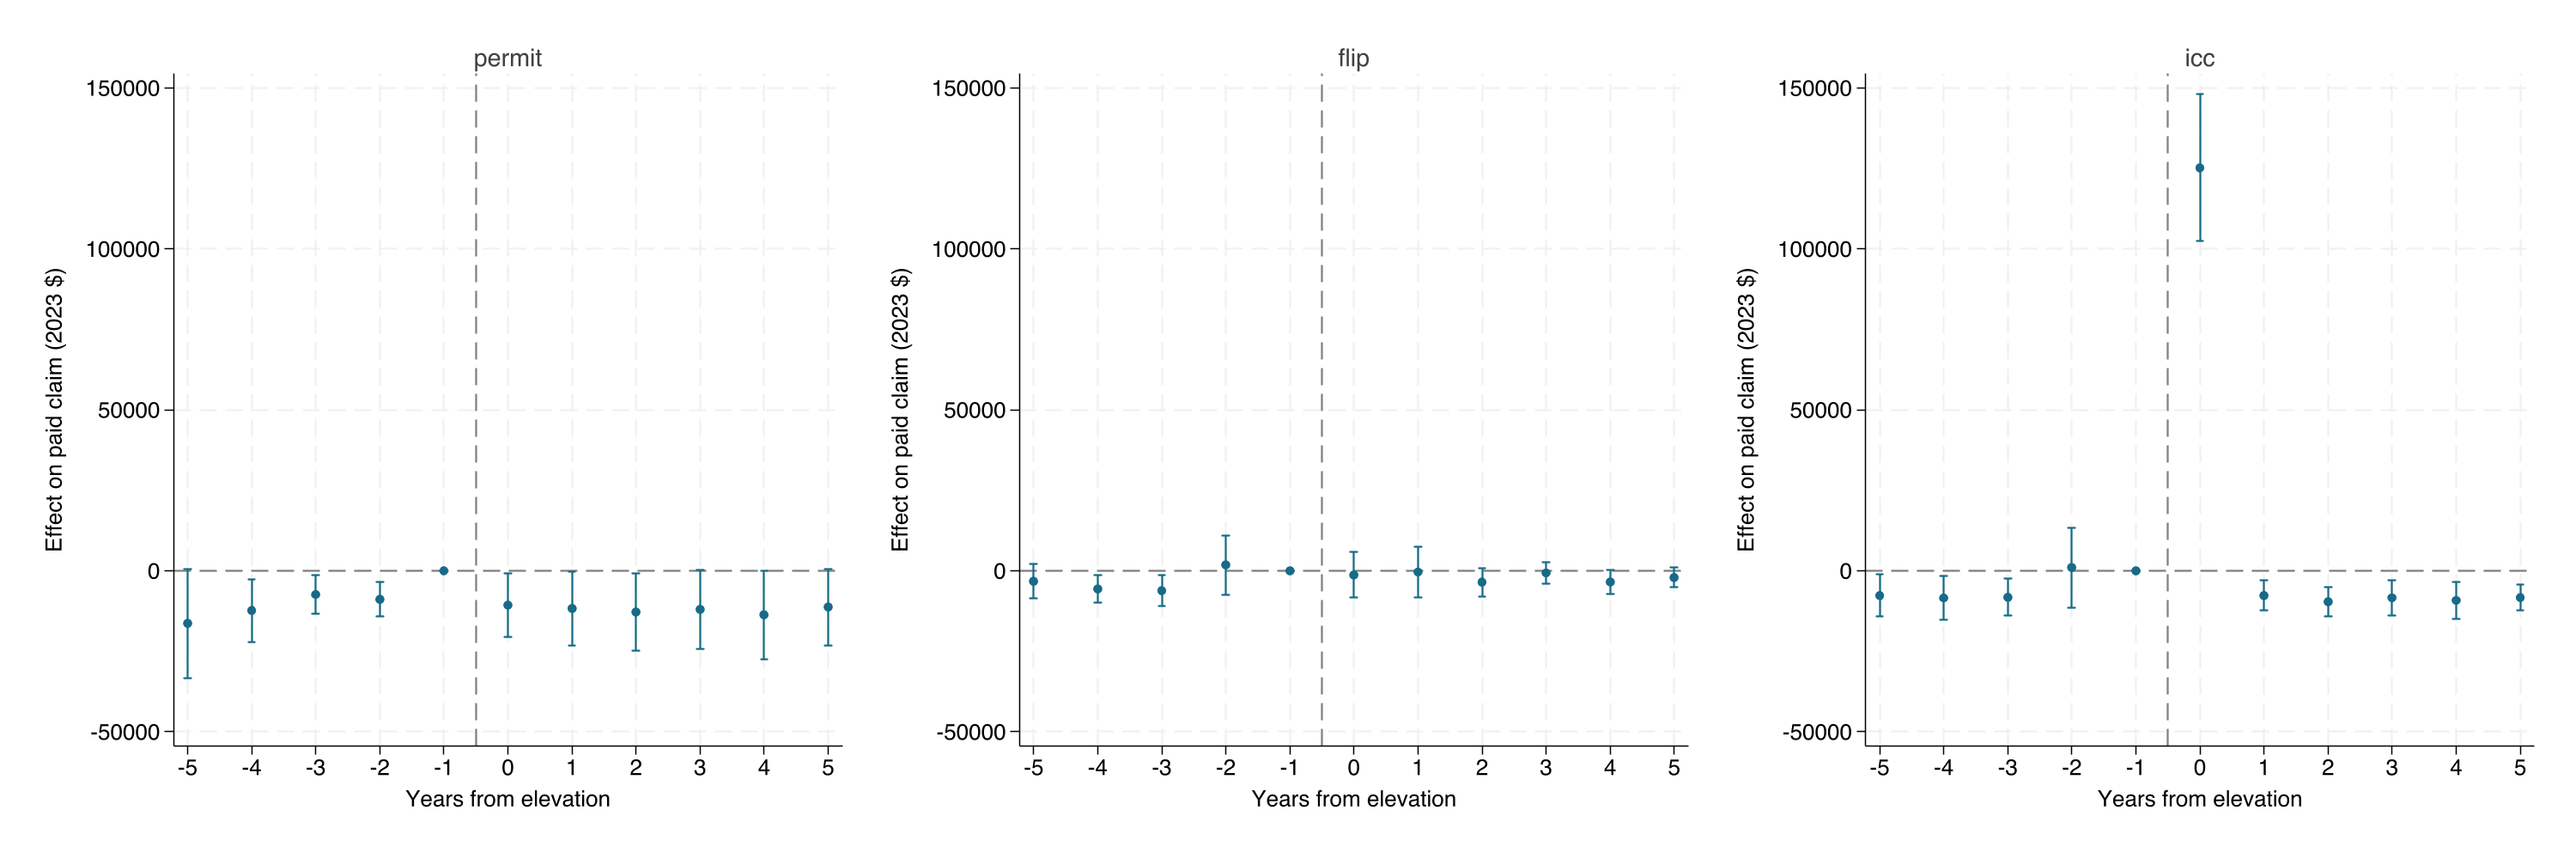
\includegraphics[width=0.98\textwidth]{es_elevation_claim_by_source.png}
\begin{itemize}
    \item The permit follows the flood (year $-1$, the reference); the ICC year is the flood itself (year 0); a flag flip is the insurer's re-rating, years after the work
    \item For no source do claims fall below their normal pre-flood level after the event: the within-home design compares average years, and the return to elevating appears only in flood years
\end{itemize}
\end{frame}

\begin{frame}{Appendix: Premiums Around the Elevation, by Source}
\centering
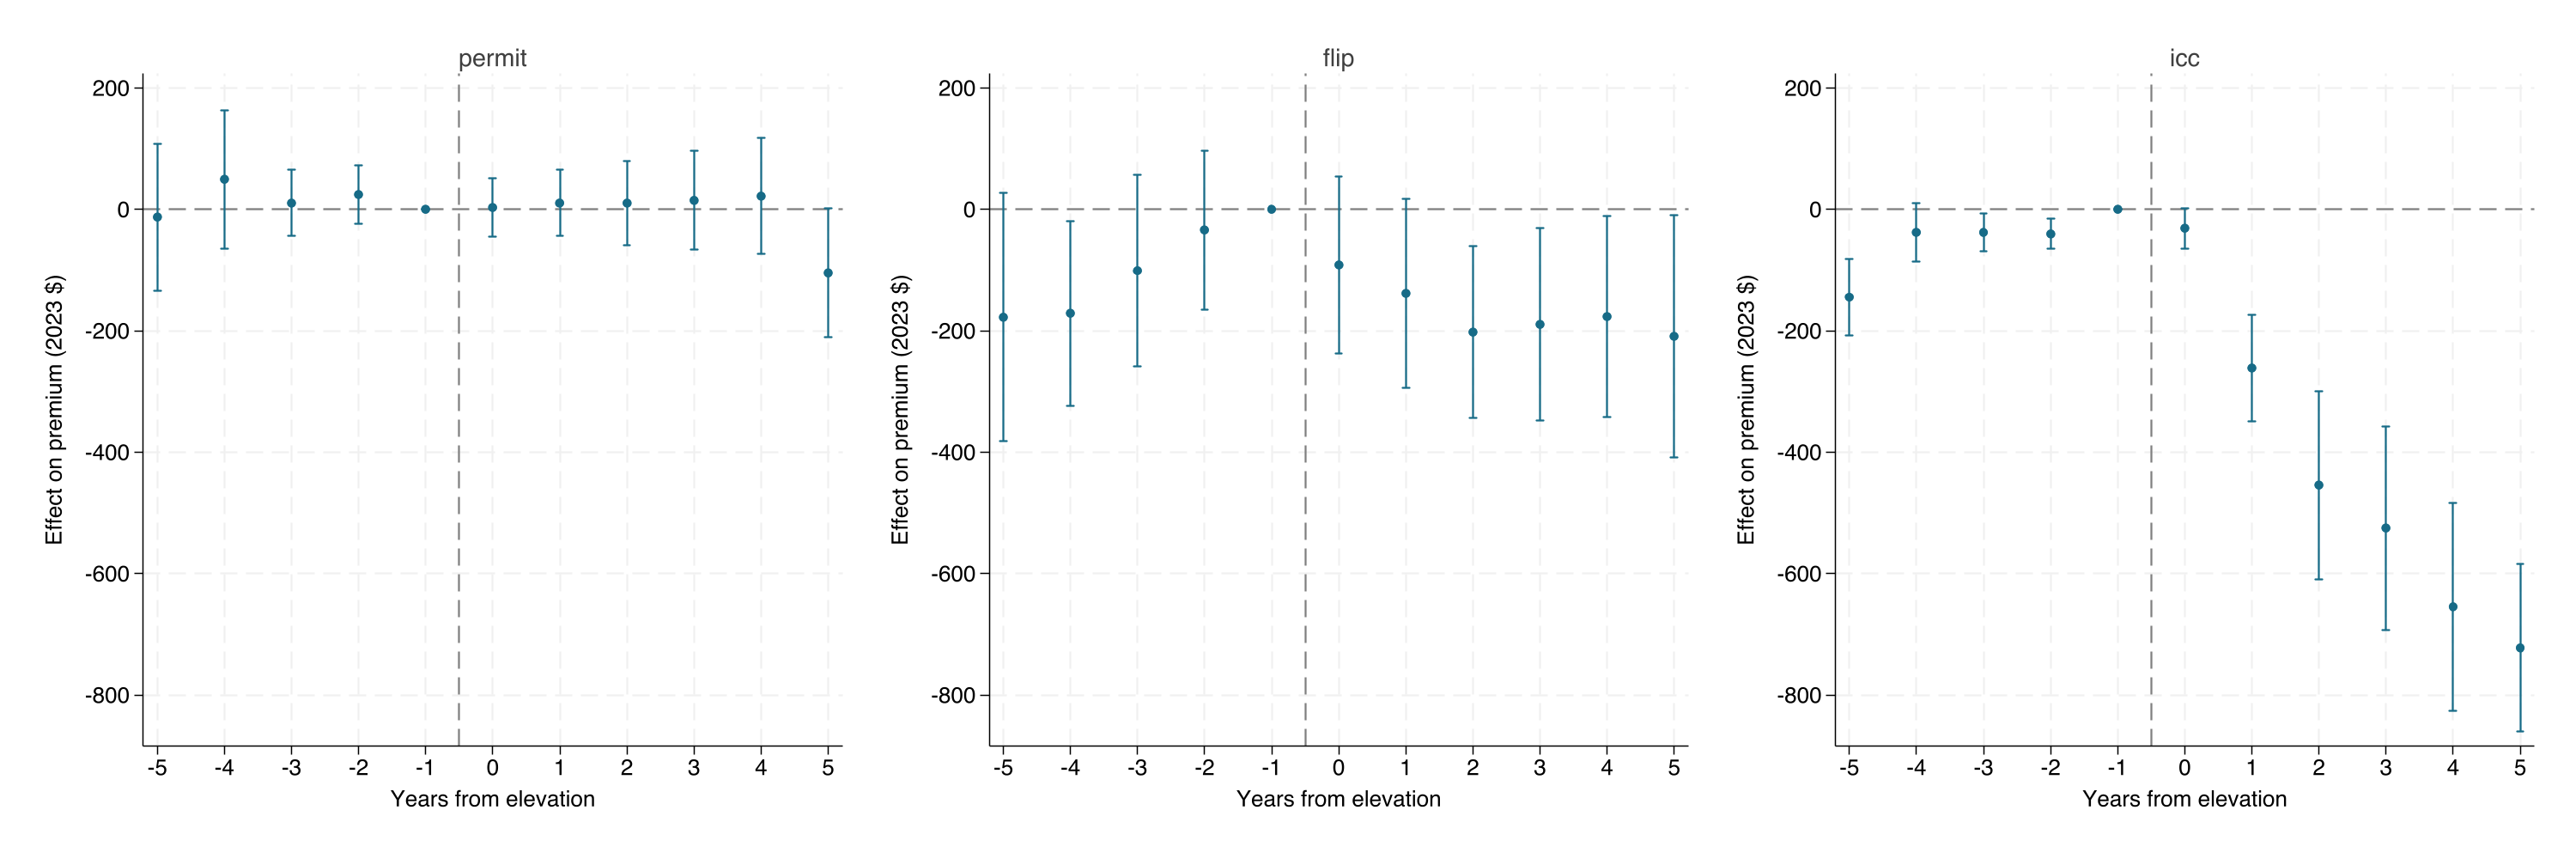
\includegraphics[width=0.98\textwidth]{es_elevation_premium_by_source.png}
\begin{itemize}
    \item Permitted homes: no change. Flag-flip and ICC homes: the premium falls after the event, with a downward pre-trend, consistent with the insurer re-rating the house rather than a return to a private investment
\end{itemize}
\end{frame}

% Figure: descriptives/scratch/hma_cost_timeseries.do -> hma_cost_cumulative_elevation.png
% (funded HMGP and FMA elevation projects, total project cost by obligation year, 2024 $).
\begin{frame}{Appendix: Federal Spending on Home Elevations}
\centering
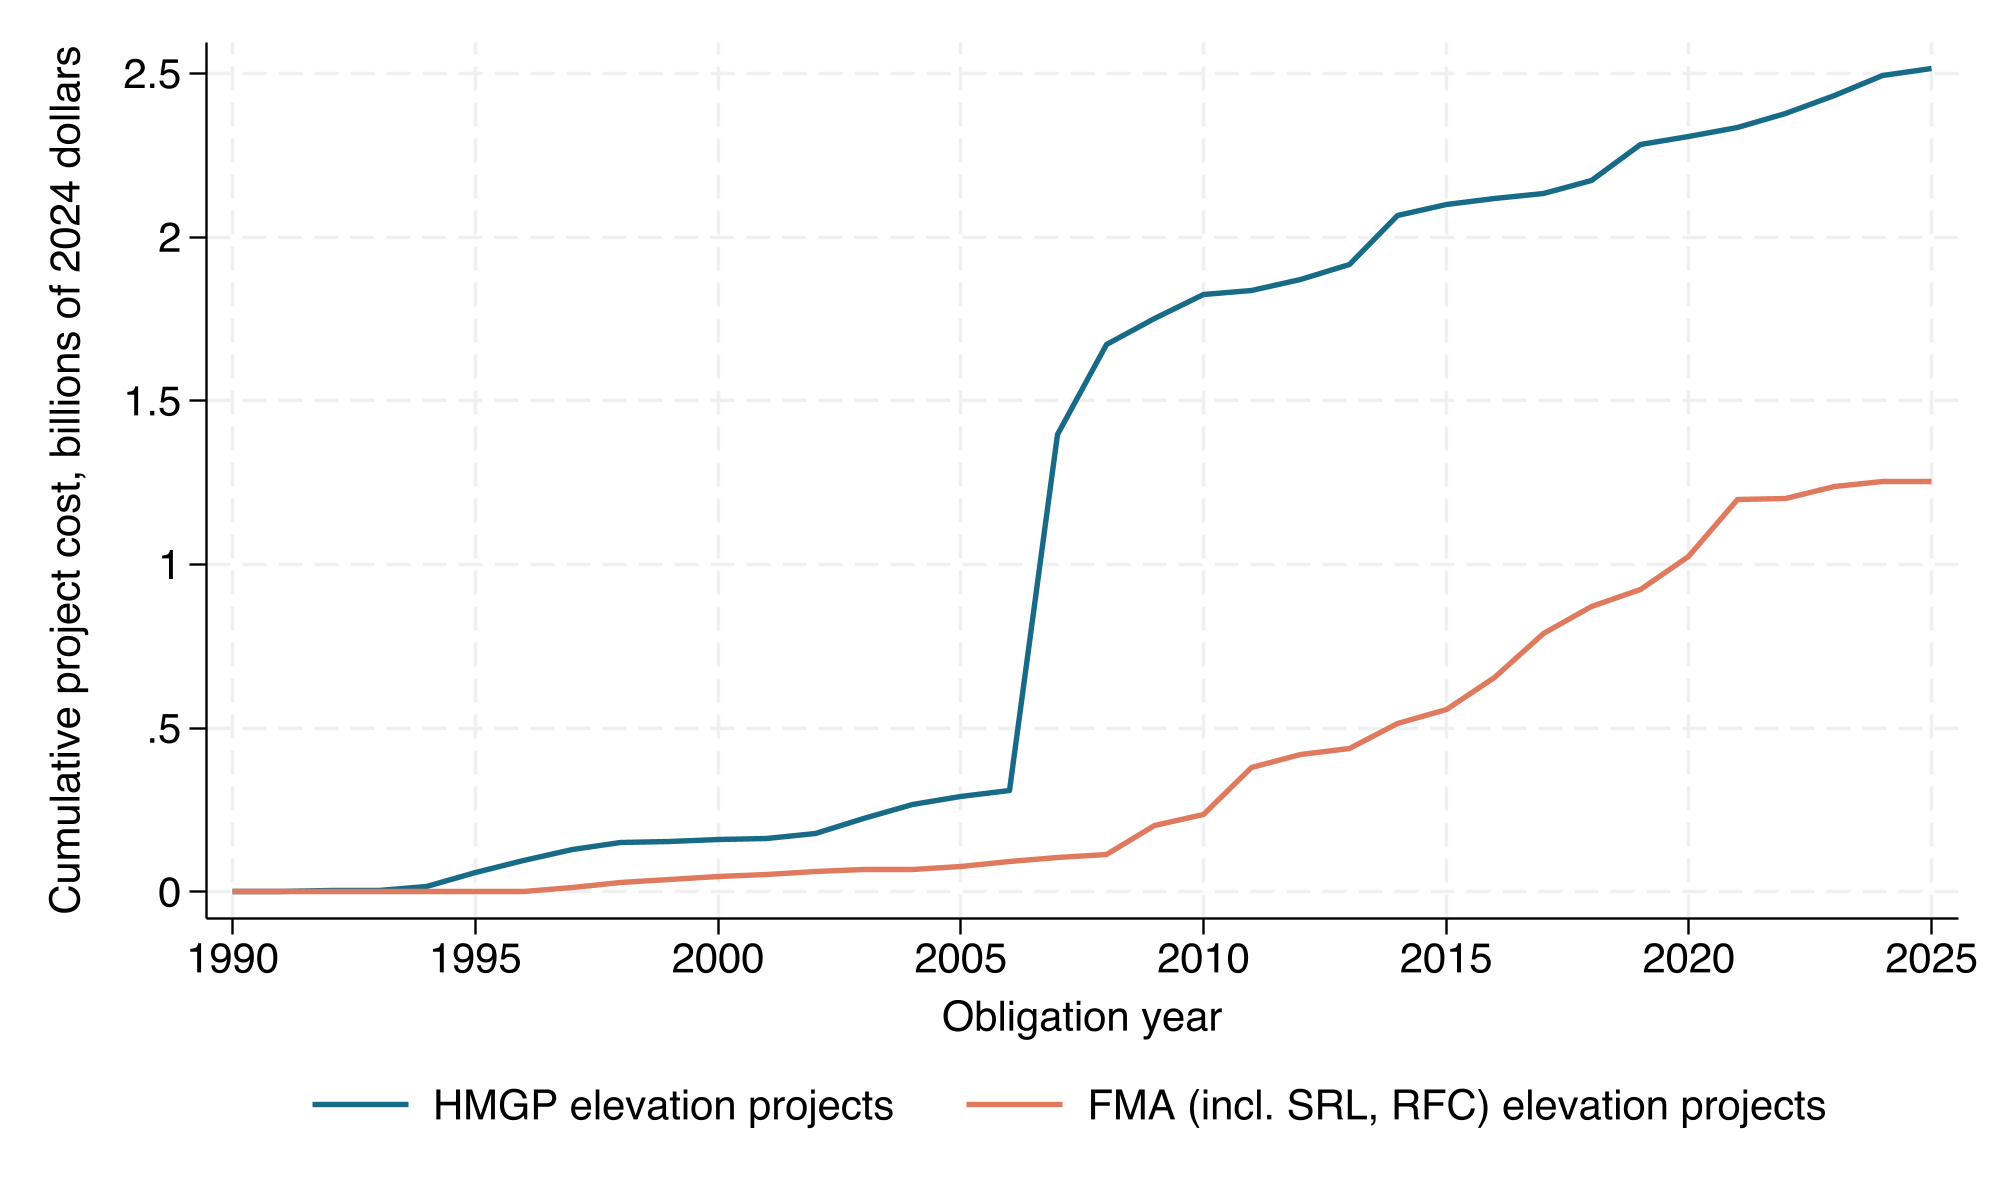
\includegraphics[width=0.72\textwidth]{hma_cost_cumulative_elevation.png}
\end{frame}

\end{document}
